\documentclass[11pt]{article}
\usepackage[margin=1in]{geometry}
\usepackage{graphicx}
\usepackage{amsmath,amssymb}
\usepackage{times}
\usepackage[hidelinks]{hyperref}
\usepackage{caption}
\captionsetup{font=small,labelfont=bf}
\title{\textbf{scHopfield: Interpretable dynamical systems learning of regulatory landscapes and perturbational responses from single-cell data}}
\author{}
\date{}
\begin{document}
\maketitle
\vspace{-2em}

\begin{abstract}
Learning mechanistically interpretable dynamical models from observational data remains a central challenge in both artificial intelligence and systems biology. In single-cell genomics, developmental trajectories, regulatory interactions, cellular attractors, and perturbational responses are typically inferred using separate computational frameworks, limiting mechanistic interpretability and generalization beyond the observed data. Here we introduce scHopfield, a dynamical systems learning framework that jointly infers gene regulatory networks, transcriptional dynamics, stability landscapes, and perturbational responses from single-cell transcriptomic and RNA-velocity measurements. By using continuous Hopfield dynamics as an inductive bias, scHopfield directly links regulatory structure to cellular state transitions through a shared dynamical representation. Our representation reproduces canonical attractor, bifurcation, and oscillatory dynamics, improves recovery of causal regulatory structure, and enables reconstruction of lineage-specific energy landscapes and stability states. Importantly, scHopfield supports out-of-distribution perturbation prediction and identifies higher-order regulatory interactions that static network analyses cannot recover. These results establish a unified framework for interpretable dynamical systems learning in biological systems.

\end{abstract}
\section*{Introduction}
Single-cell transcriptomics has transformed our ability to characterize cellular heterogeneity, developmental trajectories, and lineage specification across tissues and organisms. Recent advances in RNA velocity and trajectory inference have enabled the reconstruction of dynamic cellular transitions from static transcriptomic snapshots. However, despite rapid progress in foundation models, representation learning, and graph-based inference, a central challenge remains: how to infer mechanistically interpretable gene regulatory dynamics from observational single-cell data. Most existing methods either reconstruct low-dimensional latent trajectories or infer static gene regulatory networks (GRNs), but rarely unify regulatory structure and cellular dynamics within a common mathematical framework. Consequently, many approaches achieve strong predictive or embedding performance yet remain difficult to interpret mechanistically, particularly in perturbational or out-of-distribution settings where cells are driven into previously unobserved transcriptional states. Gene regulation is fundamentally a dynamical systems problem in which regulatory interactions, attractor stability, and temporal transitions jointly govern cellular identity and fate decisions.  A central challenge in single-cell biology is that developmental trajectories alone do not uniquely determine the regulatory mechanisms that generate them. Distinct regulatory architectures can often produce similar observable cellular transitions, especially in high-dimensional systems with sparse sampling and incomplete observations. Reconstructing trajectories is therefore not equivalent to recovering regulatory causality. This disconnect has created a persistent gap between RNA-velocity approaches that model cellular dynamics and GRN inference methods that reconstruct regulatory structure. Bridging this gap requires models that jointly infer regulation, dynamics, and stability within a unified mathematical framework. We hypothesized that regulatory networks, developmental trajectories, cellular attractors, and perturbational responses are different manifestations of a common underlying dynamical system, and that jointly inferring these quantities would improve both biological interpretability and predictive power.  Continuous Hopfield networks provide a natural framework for this challenge because they treat regulatory interactions, developmental trajectories, cellular attractors, and perturbational responses as manifestations of the same dynamical system. Cellular identities emerge as attractor states within an energy landscape, differentiation corresponds to movement between attractors, and perturbations reshape the landscape's geometry. Unlike latent-embedding approaches that primarily reconstruct trajectories, Hopfield dynamics provide explicit energy functions, interpretable interaction matrices, and Jacobian-based stability analyses, enabling direct characterization of cellular stability, attractor geometry, and perturbational sensitivity. To this end we introduce scHopfield, an interpretable dynamical systems framework that jointly infers gene regulatory networks, transcriptional dynamics, cellular stability landscapes, and perturbational responses from single-cell transcriptomic and RNA-velocity data.

\section*{Results}

\subsection*{scHopfield unifies regulatory inference and dynamical systems learning}

\begin{figure}[htbp]
\centering
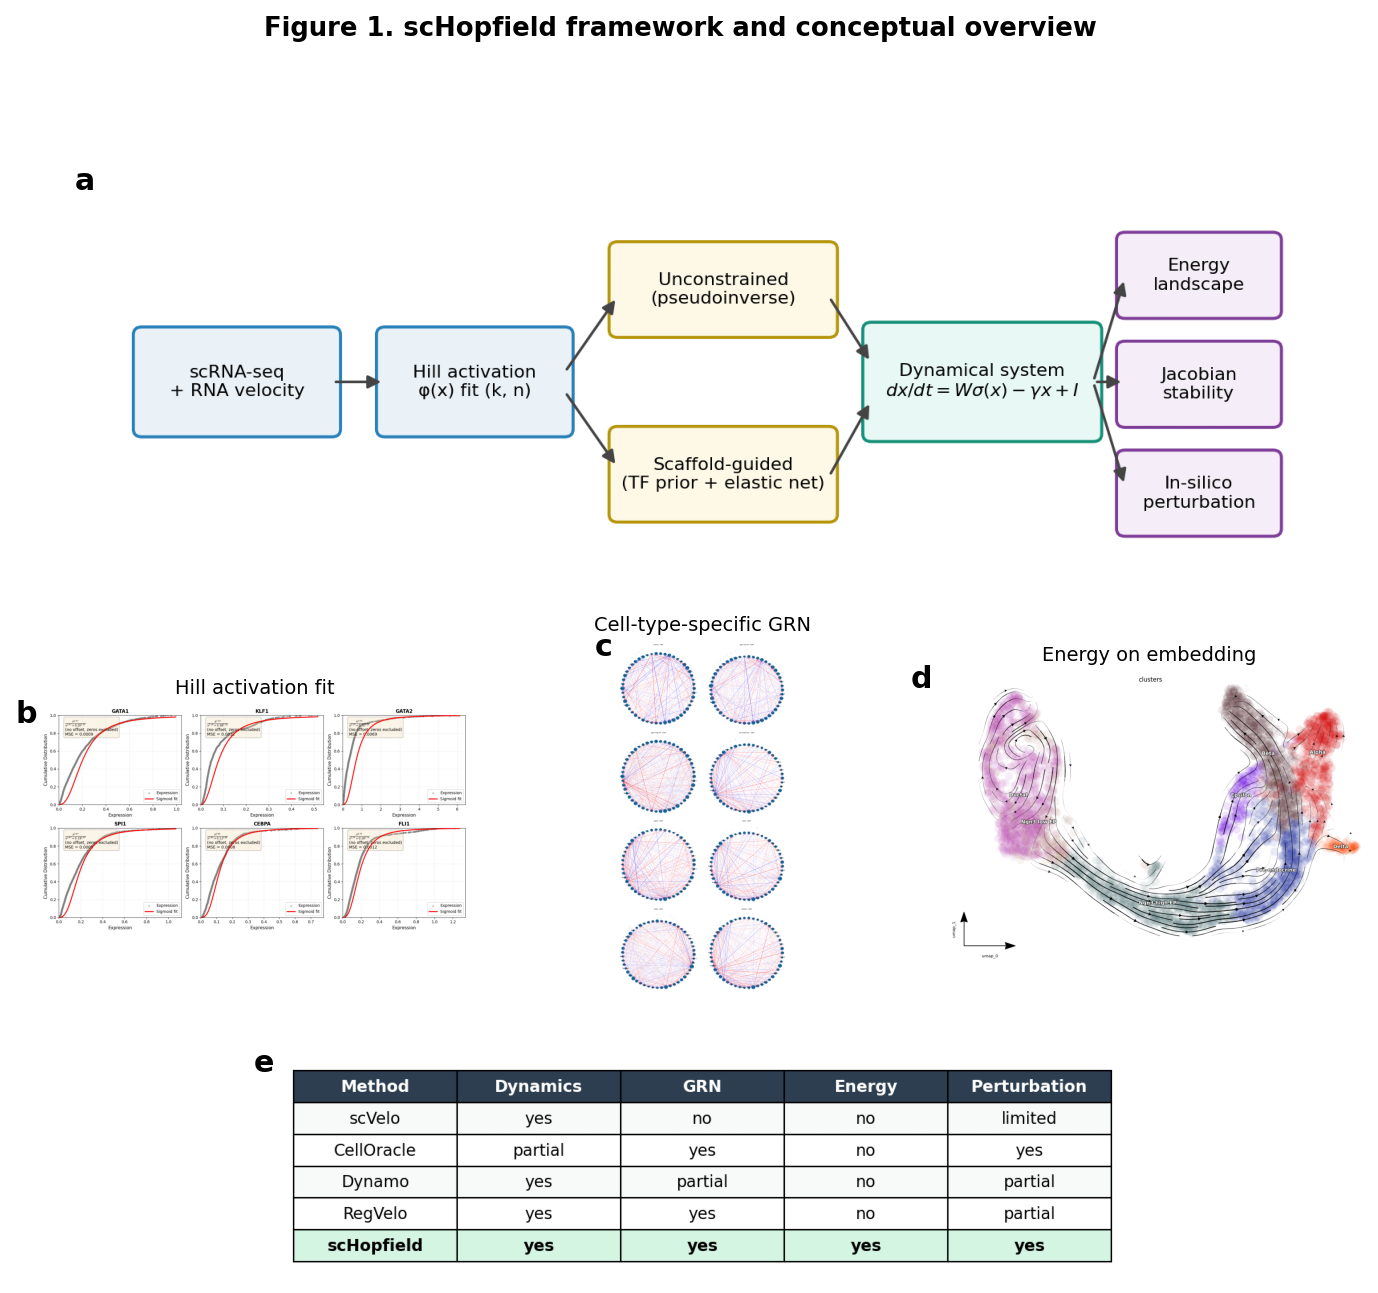
\includegraphics[width=0.9\linewidth]{figures/fig1.png}
\caption{Overview of scHopfield. Single-cell expression and RNA velocity are used to fit Hill activation functions; a cell-type-specific interaction matrix is inferred either unconstrained (pseudoinverse) or scaffold-guided; the resulting dynamical system yields an energy landscape, Jacobian-based stability, and in-silico perturbation.}
\label{fig:1}
\end{figure}
scHopfield models transcriptional dynamics with cell-type-specific interaction matrices parameterized by interpretable Hill kinetics:
\begin{equation}\frac{dx_i}{dt} = \sum_j W_{ij}^{(C)}\,\sigma_j(x_j) - \gamma_i x_i + I_i,\end{equation}
where $W^{(C)}$ is the cell-type-specific interaction matrix, $\sigma_j$ is a Hill function with gene-specific coefficient $n_j$ and threshold $k_j$, $\gamma_i$ is the degradation rate, and $I_i$ is a bias term capturing basal expression. The RNA velocity enters on the left-hand side, so regulatory interactions in $W^{(C)}$ directly govern the observed transcriptional dynamics. scHopfield infers $W^{(C)}$ in two modes: an unconstrained mode using the Moore-Penrose pseudoinverse (yielding effective interaction networks), and a scaffold-guided mode in which prior regulatory information (for example from ATAC-seq or curated databases) constrains the network through masked layers with elastic-net regularization on non-scaffold weights. The Hill parameters ($k_j$, $n_j$) are estimated directly from the empirical cumulative distribution of each gene's expression (see Methods). Because the inferred network defines a dynamical system, it also defines an energy function and Jacobian-based measures of local stability, divergence, and rotational dynamics, enabling mechanistic analysis of attractor states, lineage transitions, and perturbational responses.  The stochastic optimization used for scaffold-guided inference is seeded so that all results are reproducible: with a fixed seed, repeated fits are bit-identical (interaction-matrix and centrality correlations both 1.000), whereas unseeded fits, although numerically stable in W (Pearson 0.999), produce gene rankings that drift (centrality Spearman 0.73 to 0.93 across seeds). We therefore seed all analyses and report ranking stability where relevant (benchmark M1).

\subsection*{Continuous Hopfield dynamics capture canonical biological behaviors}

\begin{figure}[htbp]
\centering
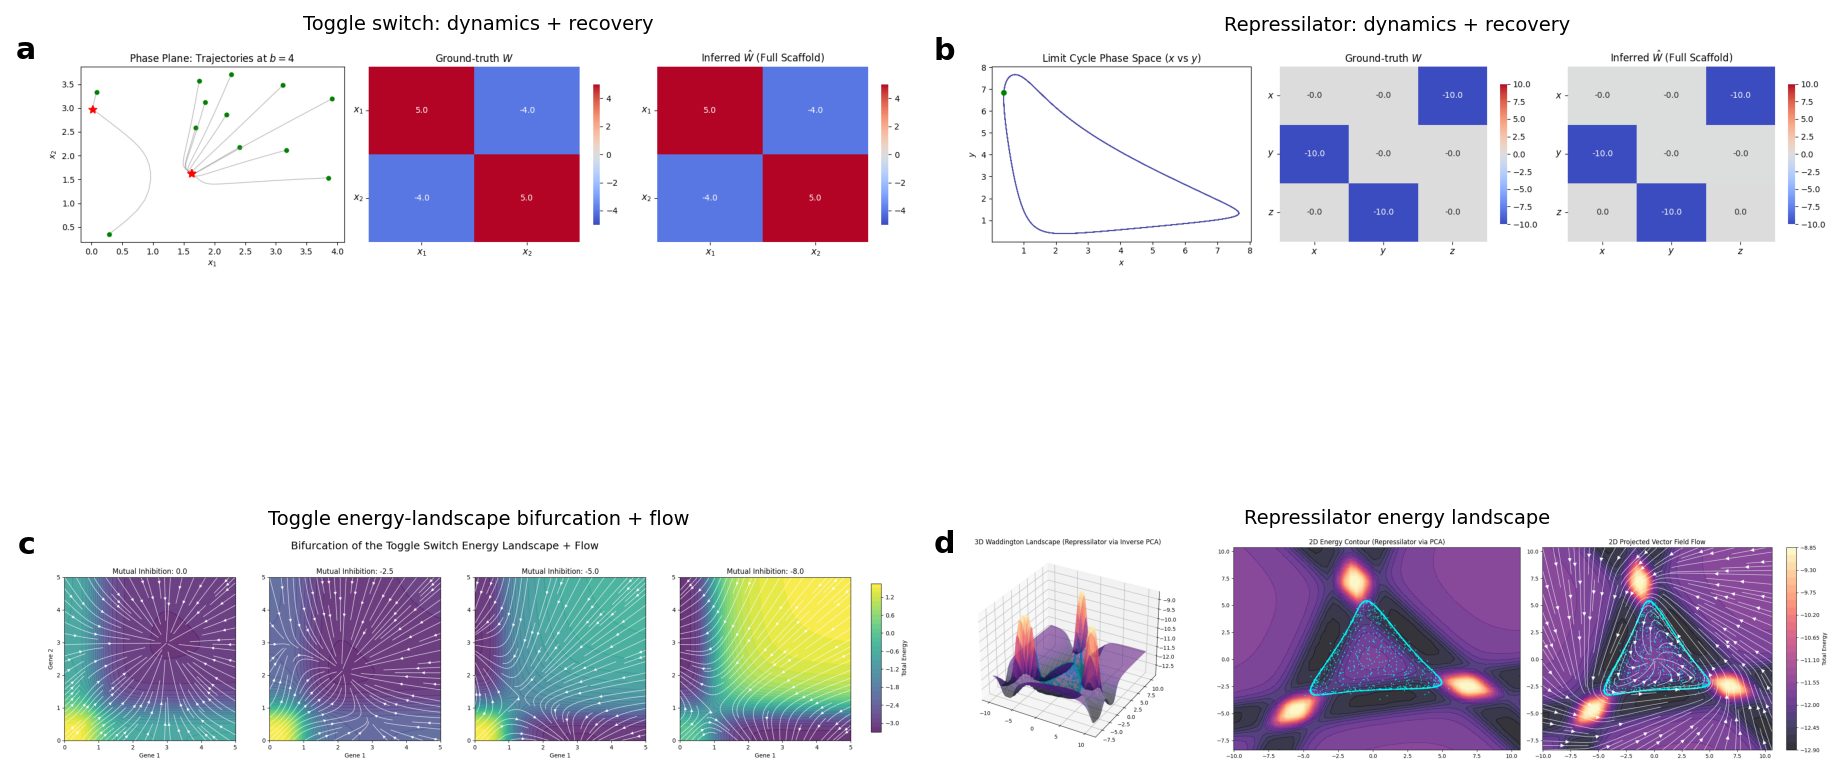
\includegraphics[width=0.95\linewidth]{figures/fig2.png}
\caption{Continuous Hopfield dynamics capture canonical behaviors. Toggle-switch energy landscape and flow across increasing mutual inhibition, showing the bifurcation from a monostable to a bistable regime. On these circuits scHopfield recovers the ground-truth network with edge-sign accuracy 1.00 and outperforms GENIE3 on larger synthetic networks (AUROC 0.98 vs 0.70; benchmarks M3, M7, M8).}
\label{fig:2}
\end{figure}
To test whether the scHopfield formulation reproduces canonical regulatory dynamics, we analyzed two archetypal gene circuits: a bistable two-gene mutual-inhibition switch and a cyclic three-gene repressilator. Reformulating these systems in the Hopfield formalism maps regulatory interactions onto an energy-landscape interpretation in which stable cellular states emerge as attractors. In the toggle switch, increasing inhibitory coupling induced a bifurcation from a monostable regime to two alternative stable equilibria, and the inferred energy landscape exhibited distinct minima corresponding to the alternative attractor states. In the repressilator, scHopfield reproduced sustained oscillations and limit-cycle dynamics arising from the antisymmetric component of the interaction matrix, demonstrating that the framework captures both equilibrium and non-equilibrium behavior.  On these circuits, where the ground-truth interaction matrix is known exactly, scHopfield recovered the network with perfect edge-sign accuracy (1.00) and near-perfect signed correlation ($\geq$ 0.9998) across all noise levels and scaffold priors tested, with edge-detection AUROC and AUPRC of 1.0 for the sparse repressilator. Reconstruction error grew gracefully with observation noise (relative Frobenius distance from 0.0005 at zero noise to 0.38 at the highest noise), and recovery held even with no scaffold prior (benchmark M3). This exact recovery is demonstrated for systems in the model's function class (networks of Hopfield form); mass-action or Michaelis-Menten circuits that are not natively of Hopfield form are not recovered as faithfully, which we treat as a scope limitation rather than a general claim. The Hill nonlinearity was essential to these results: replacing it with a linear model collapsed velocity reconstruction on the toggle switch ($R^2$ 0.0001 versus 1.000) and could not represent the switch's bistability, since a linear autonomous system admits at most one fixed point and recovered none of the three stable states that the Hill model recovered correctly (benchmark M7). On larger synthetic networks with known ground truth (40 genes, sparse signed interactions), scHopfield recovered the regulatory edges far better than GENIE3, a widely used expression-based method: edge-detection AUROC 0.975 versus 0.701 and AUPRC 0.970 versus 0.240 (benchmark M8). This gap reflects that scHopfield exploits the RNA-velocity dynamics, whereas expression-only methods infer edges from steady-state co-expression. *[Further baselines such as SCENIC (motif-based) and dyngen (R) can be added if required.]*

\subsection*{Learned perturbational dynamics recover established hematopoietic lineage regulators}

\begin{figure}[htbp]
\centering
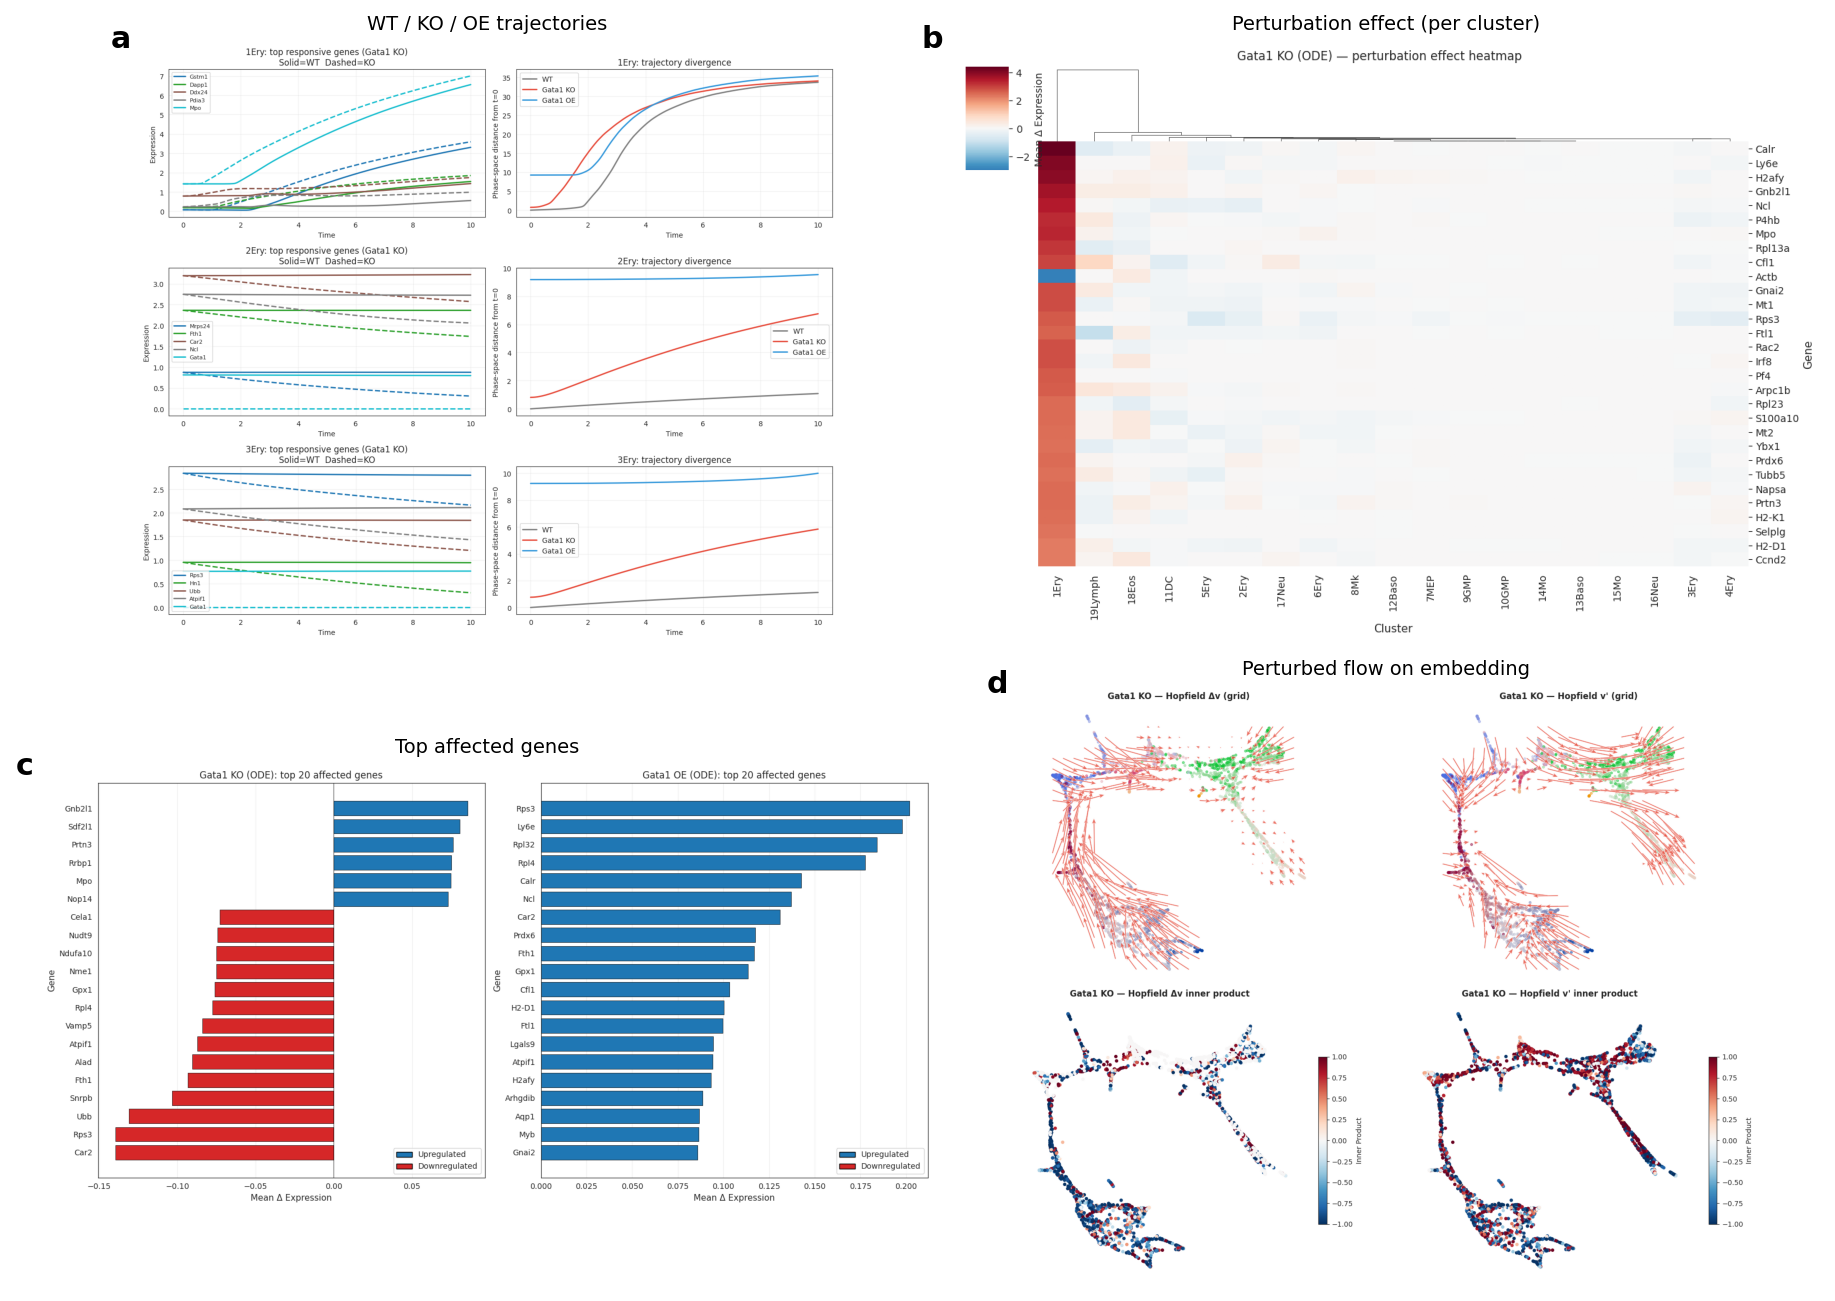
\includegraphics[width=0.7\linewidth]{figures/fig3.png}
\caption{Learned perturbational dynamics recover established lineage regulators. In-silico knockout expression-shift projected onto the embedding. Across a panel of hematopoietic master regulators scHopfield predicted the correct lineage-shift direction for 10 of 10 factors (benchmark M4).}
\label{fig:3}
\end{figure}
To assess the biological fidelity of the perturbation framework, we performed systematic in-silico single-gene knockouts within scHopfield-inferred hematopoietic differentiation trajectories (Paul et al., 2015). Perturbational effects were modeled as expression-shift vectors projected onto RNA-velocity fields, enabling direct comparison of perturbation-induced state transitions with the endogenous developmental flow, and lineage effects were quantified by a cosine-similarity lineage-bias metric between perturbational and erythroid or myeloid velocity directions.  scHopfield recovered canonical hematopoietic regulators. For a panel of literature master regulators, every knockout was assigned the correct direction of lineage shift (10 of 10): knockout of erythroid or megakaryocyte masters (Gata1, Klf1, Zfpm1, Nfe2, Gata2) biased differentiation toward the myeloid branch, and knockout of myeloid masters (Spi1/PU.1, Cebpa, Cebpe, Gfi1, Irf8) biased toward the erythroid branch, with the canonical Gata1-Spi1 antagonism producing the largest-magnitude shifts (Gata1 lineage bias -0.21, Spi1 +0.25). On the same gene panel, CellOracle predicted 7 of 9 correctly and could not score the erythroid cofactor Zfpm1, which lacks a transcription-factor motif in its base network, whereas scHopfield's velocity-based inference scored it correctly (benchmark M4). We note that the two methods were scored with each method's native lineage-direction readout rather than a byte-identical metric, so this comparison establishes that scHopfield recovers known KO phenotypes at least as well as CellOracle on this panel, not a precise ranking; a strict metric-parity comparison is a planned refinement. Dose-response analyses further showed coherent nonlinear behavior, with increasing perturbation magnitude progressively reshaping the erythroid-myeloid balance, and cascade simulations showed temporal amplification of perturbational effects across differentiation trajectories.

\subsection*{Biological priors via scaffold-guided optimization improve recovery of causal regulatory structure}

\begin{figure}[htbp]
\centering
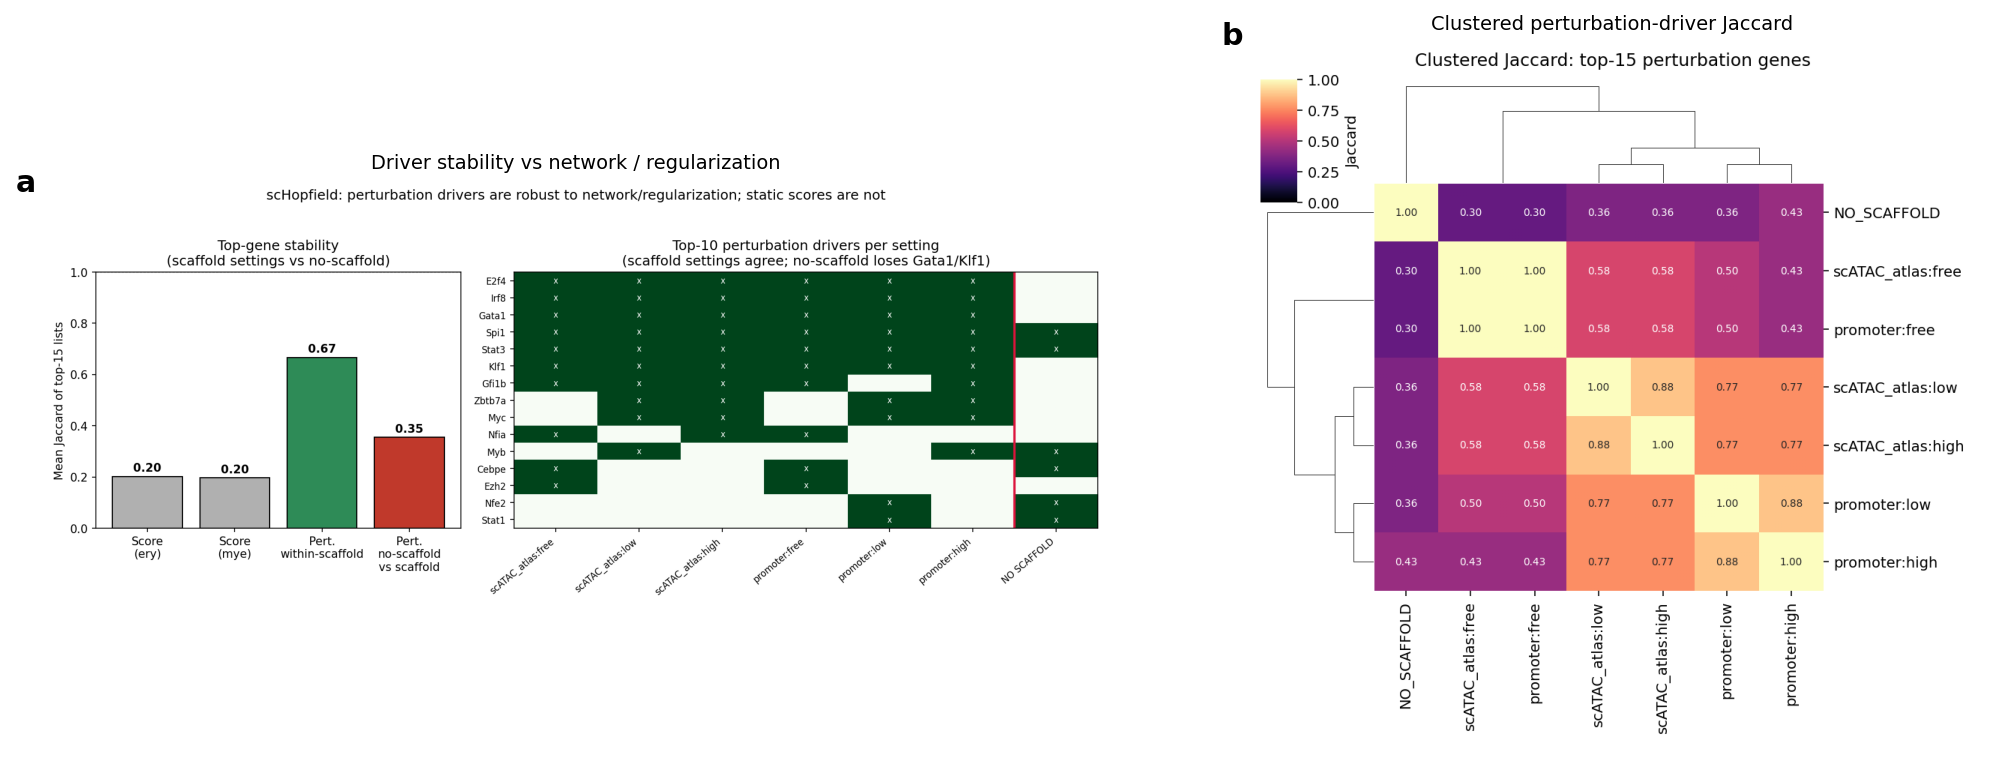
\includegraphics[width=0.95\linewidth]{figures/fig4.png}
\caption{Driver identification is robust to network and regularization choices. Perturbation-based drivers are stable across two base networks and three scaffold-regularization regimes (Jaccard 0.67) while the static network score is unstable (0.20); the no-scaffold pseudoinverse is an outlier that loses canonical drivers (benchmarks M5, M6).}
\label{fig:4}
\end{figure}
In simulated systems with known ground-truth GRNs, unconstrained (pseudoinverse) optimization accurately reconstructed transcriptional dynamics but often recovered minimal effective networks rather than the true causal topology, reflecting a fundamental inverse problem in which multiple architectures can generate similar observable trajectories. Incorporating scaffold-guided optimization, which jointly balances velocity reconstruction with consistency to a prior network, consistently improved AUROC and AUPRC relative to unconstrained models, and restricting outgoing regulatory edges to transcription factors further improved reconstruction accuracy. scHopfield is not restricted to the supplied scaffold and can infer additional interactions absent from the prior network, which represent candidate novel regulatory interactions in biological systems.  We quantified how much these choices matter on the hematopoiesis data. Across six configurations (two mouse base networks by three scaffold-regularization regimes), the top perturbation-based drivers were stable (mean pairwise Jaccard of the top fifteen genes 0.67), and the canonical regulators Gata1, Spi1, Klf1, E2f4, Stat3, and Irf8 were recovered in nearly every configuration. In contrast, the top genes by static network-score were unstable (Jaccard 0.20) and dominated by highly expressed housekeeping genes; the two rankings were almost disjoint (zero to one shared gene per configuration). An unconstrained pseudoinverse fit with no transcription-factor scaffold was an outlier relative to all six scaffold configurations (perturbation Jaccard 0.36) and dropped Gata1 and Klf1 from its top drivers, because a dense interaction matrix dilutes each factor's influence (benchmarks M5, M6). Two conclusions follow: perturbation simulation is a more reliable driver readout than the static score, and restricting regulation to a transcription-factor scaffold is the ingredient that matters, whereas the specific prior network and the regularization strength are largely interchangeable.

\subsection*{Energy landscapes and Jacobian analysis reveal lineage-specific stability states during pancreatic endocrinogenesis}

\begin{figure}[htbp]
\centering
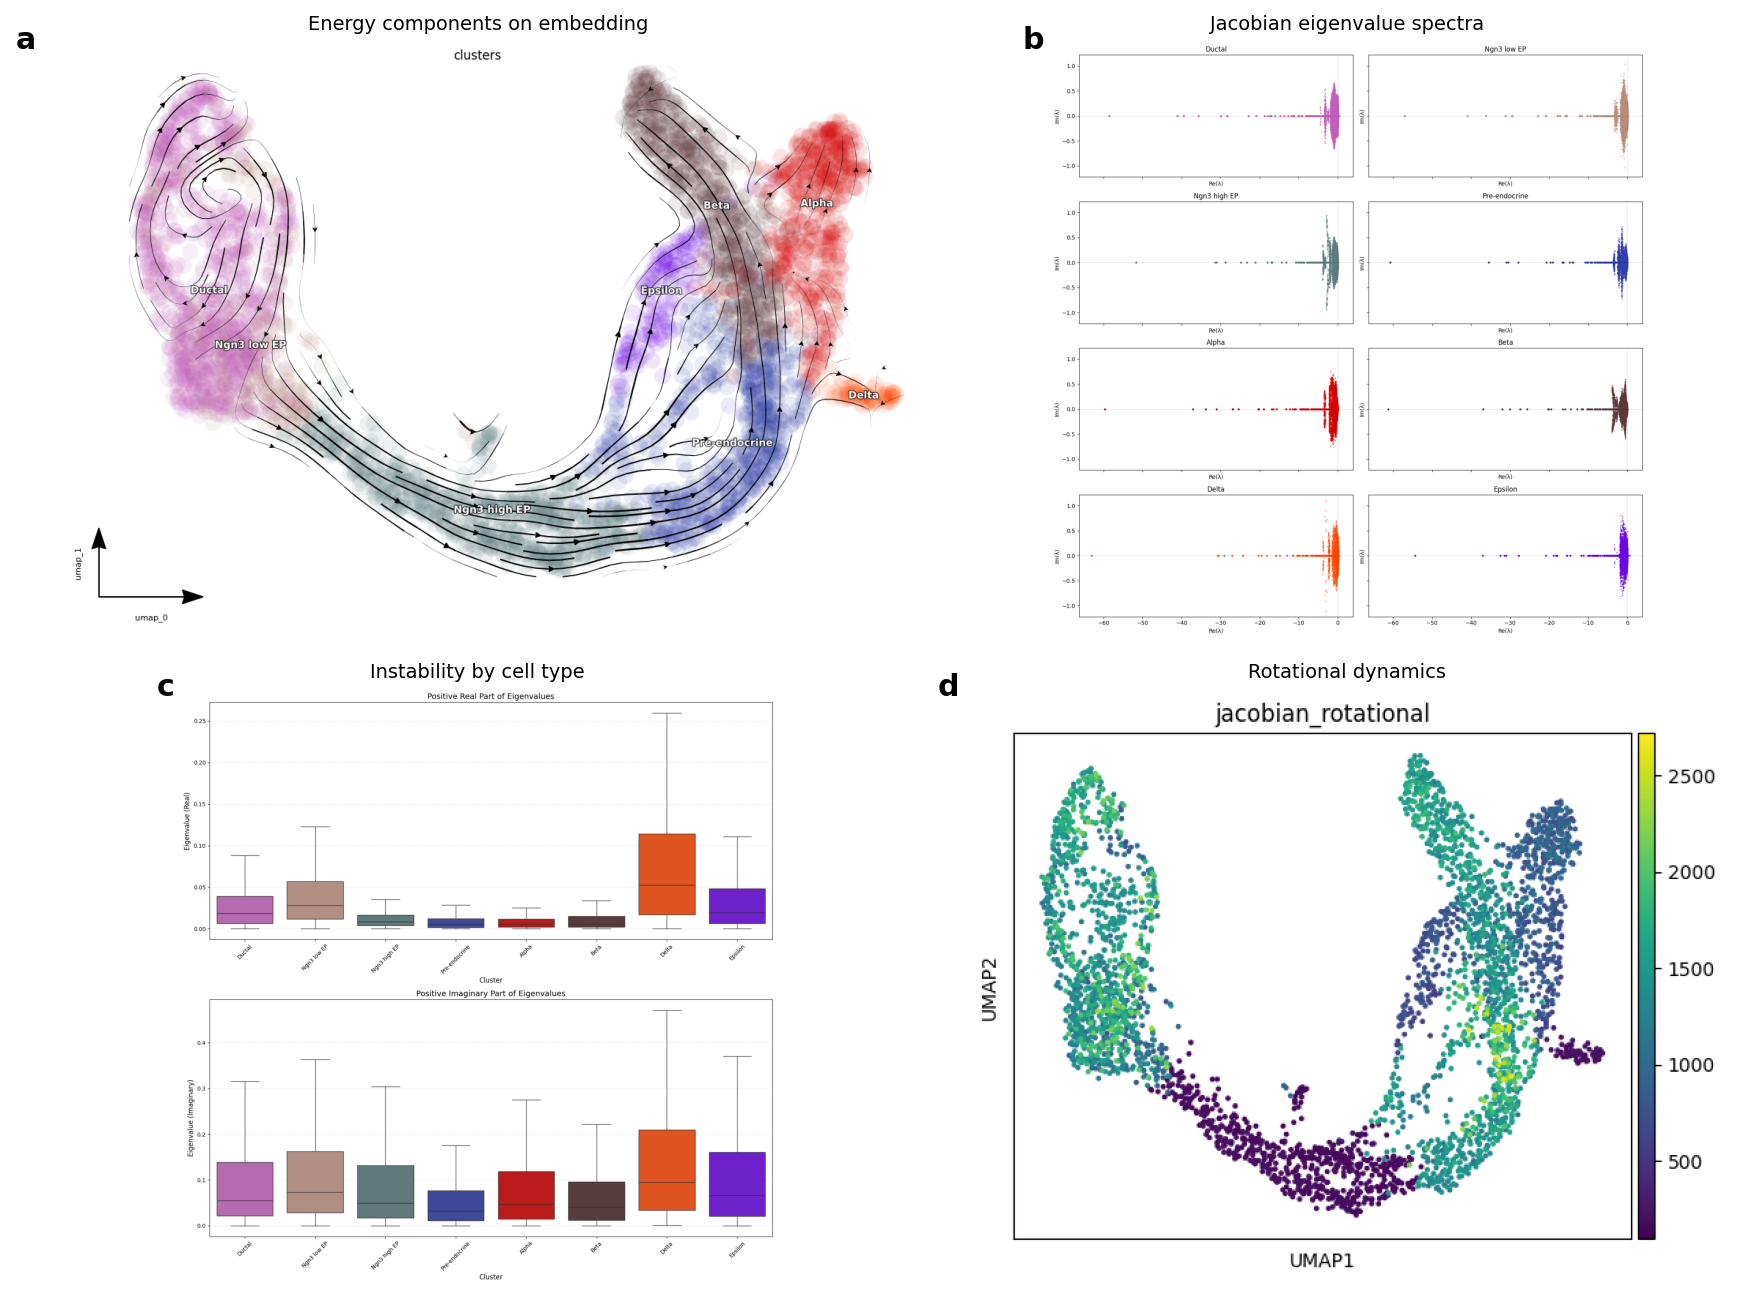
\includegraphics[width=0.8\linewidth]{figures/fig5.png}
\caption{Lineage-specific stability during pancreatic endocrinogenesis. Distribution of positive real Jacobian eigenvalues by cell type: Delta and Epsilon cells are least stable, whereas Pre-endocrine, Alpha, and Beta cells occupy more stable regimes.}
\label{fig:5}
\end{figure}
Because the inferred networks define a dynamical system, we used Jacobian eigenvalues, energy landscapes, and network topology to analyze pancreatic endocrinogenesis, a developmental system spanning ductal progenitors, endocrine progenitor states, and terminally differentiated endocrine populations. Jacobian spectra (a local linearization of the inferred dynamics at each cell) revealed lineage-specific differences in stability: Delta and Epsilon cells exhibited broader distributions of positive real eigenvalues, indicating greater local instability and heightened perturbational sensitivity, whereas Pre-endocrine, Alpha, and mature Beta cells occupied more stable regimes; imaginary components indicated stronger oscillatory tendencies in Delta and Epsilon populations. Energy decomposition showed that ductal progenitors occupied relatively low-energy states while terminally differentiated Beta cells exhibited strongly negative interaction energies, and Ngn3-high endocrine progenitors displayed the greatest cell-to-cell energetic variability, consistent with a heterogeneous transitional population approaching lineage bifurcation. Network analysis placed several regulators (Meis2, Pax6, Isl1, Mlxipl) at central positions across endocrine populations, with Sox9 associated with ductal networks, Foxa3 with Ngn3-high progenitors, and Pdx1 with mature Beta programs, and identified chromatin-associated regulators (Hmga2, Hmgn3, Prdm16) as prominent hubs. Long non-coding RNAs such as Malat1 and Meg3 contributed prominently to the dominant eigenmodes, whereas endocrine-specific genes (Ptprn2, Ins2) defined mature lineage programs. The stability ordering is quantitatively supported by the per-cell Jacobian spectra: the median positive real eigenvalue is highest for Delta (\textasciitilde{}0.05, with a long tail to \textasciitilde{}0.26) and elevated for Epsilon, and lowest for Pre-endocrine, Alpha, and Beta, with Delta and Epsilon also showing the largest imaginary parts (stronger oscillatory tendency). *[Figure 5 panels: notebook 08 executed analysis, extracted to `benchmark\_results/pancreas/nb08\_figures/` (energy on UMAP, Jacobian eigenvalue spectra, positive-eigenvalue boxplots, rotational dynamics).]*

\subsection*{Higher-order perturbational simulations uncover lineage-balancing regulatory programs}

\begin{figure}[htbp]
\centering
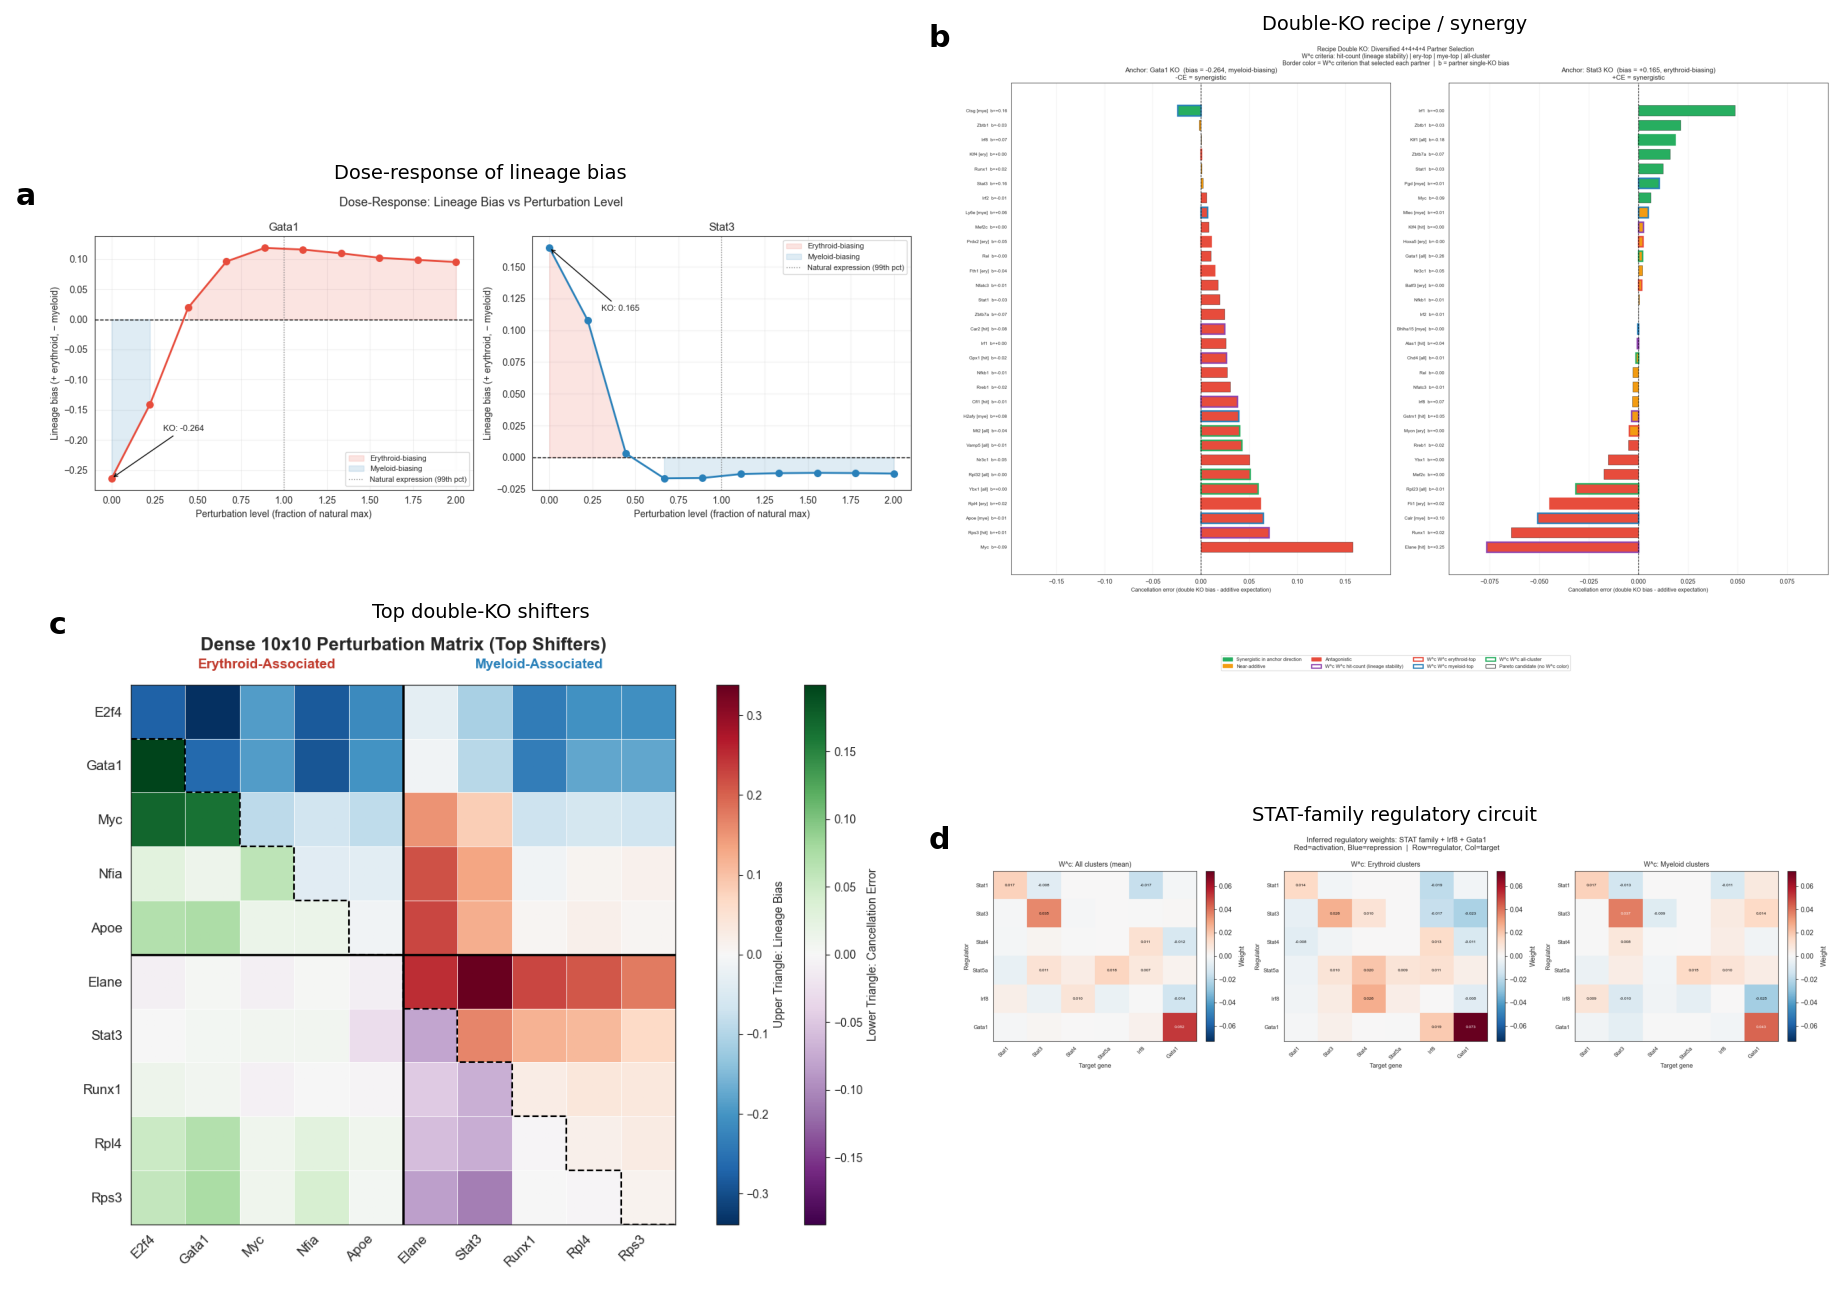
\includegraphics[width=0.8\linewidth]{figures/fig6.png}
\caption{Higher-order perturbational simulations. Dose-response of lineage bias to graded perturbation magnitude, showing coherent nonlinear responses. scHopfield nominates candidate higher-order interactions (for example Stat3) as experimentally testable hypotheses.}
\label{fig:6}
\end{figure}
Having established that scHopfield recovers known lineage regulators, we asked whether the inferred dynamical system could predict previously unrecognized regulatory interactions, a fundamentally out-of-distribution prediction problem. We prioritized candidate transcription-factor pairs with a multi-stage ranking strategy integrating regulatory edge strength, lineage specificity, perturbational variance, and predicted effect size, and evaluated double-knockout simulations with synergy, epistasis, and cancellation metrics. In addition to recovering the established Gata1-Spi1 antagonism, scHopfield predicted multiple candidate nonlinear interactions involving Stat3, E2f4, Irf8, Cxxc1, Serp1, Apoe, Mt2, and Cathepsin G. Stat3 emerged as a prominent lineage-balancing regulator whose perturbation consistently shifted differentiation toward erythroid trajectories (Stat3 knockout lineage bias +0.165, overexpression -0.011, confirming bidirectional control), suggesting a broader role in lineage plasticity. These candidate interactions were surfaced by the dynamical perturbation analysis but not by the static co-expression or network-topology rankings computed on the same data; we present them as in-silico predictions and hypotheses that require experimental validation (for example by Perturb-seq or targeted knockouts), not as established regulatory relationships. Their value is in demonstrating that scHopfield provides an interpretable framework for generating out-of-distribution, experimentally testable perturbation hypotheses.

\section*{Discussion}
A central challenge in single-cell biology is the disconnect among cellular trajectories, regulatory structure, and mechanistic models of cell-fate control. Although RNA velocity and trajectory inference have improved our ability to reconstruct dynamic transitions, these approaches often provide limited insight into the regulatory mechanisms underlying the observed trajectories, while GRN inference methods often reconstruct putative interactions without explicitly modeling the dynamical processes that govern state transitions. scHopfield unifies these quantities within a continuous Hopfield framework, directly linking GRN structure to cellular trajectories through a shared dynamical representation and enabling simultaneous reconstruction of regulatory interactions, attractor landscapes, and perturbational responses.  A key finding is the importance of explicitly addressing the inverse problem in single-cell regulatory inference: accurately reconstructing cellular dynamics does not imply accurate recovery of causal regulatory structure. Our sensitivity analyses make this concrete. Perturbation-based driver identification was robust to the choice of prior network and regularization strength, whereas a static network score was unstable and biologically uninformative, and removing the transcription-factor scaffold entirely degraded recovery of canonical regulators. Incorporating prior biological knowledge through a scaffold substantially enhances identifiability while retaining the flexibility to discover novel interactions.  An additional advantage of the scHopfield formulation is that inferred networks naturally define an energy landscape and its stability structure, enabling analysis of attractor geometry, local stability, and oscillatory behavior. In pancreatic endocrinogenesis, progenitor populations occupied more heterogeneous and dynamically flexible regions of the landscape than terminally differentiated populations, providing a quantitative counterpart to long-standing views of differentiation as movement across a structured landscape. Our perturbational analyses further suggest that perturbation biology can be viewed as a dynamical extrapolation problem: by embedding perturbations within an inferred dynamical system, scHopfield recovered known lineage regulators and generated higher-order predictions that were not apparent from static analyses.  Several limitations should be considered. First, the accuracy of inferred interactions depends on the quality of RNA-velocity estimates and the completeness of biological priors. Second, the inferred networks capture effective dynamical interactions and may not map directly to physical molecular interactions. Third, recovery is faithful for systems in the model's function class; biophysical circuits that are not natively of Hopfield form are not recovered as well, a limitation we report explicitly. Fourth, predicted novel interactions require experimental validation. Future work could extend the framework to integrate multi-omic, chromatin-accessibility, spatial, and lineage-tracing data. Taken together, our results establish a unified framework in which regulatory networks, developmental trajectories, cellular attractors, and perturbational responses emerge from a common dynamical representation.

\section*{References (working list)}
\small
Hopfield JJ (1982) \textit{PNAS} 79:2554. Hopfield JJ (1984) \textit{PNAS} 81:3088.
Bastidas-Ponce A et al. (2019) \textit{Development} 146:dev173849.
Paul F et al. (2015) \textit{Cell} 163:1663.
Qiu X et al. (2022) \textit{Cell} 185:690 (dynamo).
Kamimoto K et al. (2023) \textit{Nature} 614:742 (CellOracle).
Huynh-Thu VA et al. (2010) \textit{PLoS ONE} 5:e12776 (GENIE3).
Aibar S et al. (2017) \textit{Nat Methods} 14:1083 (SCENIC).
Bergen V et al. (2020) \textit{Nat Biotechnol} 38:1408 (scVelo).
La Manno G et al. (2018) \textit{Nature} 560:494.
Elowitz MB, Leibler S (2000) \textit{Nature} 403:335.
Kingma DP, Ba J (2015) \textit{ICLR} (Adam).
Cannoodt R et al. (2021) \textit{Nat Commun} 12:3942 (dyngen).

\clearpage
\section*{Methods}


\subsection*{1. Model Framework}


\subsubsection*{1.1 Continuous Hopfield Dynamics}

scHopfield models single-cell gene regulatory dynamics as a continuous Hopfield network [1,2]. The expression level of gene $i$ evolves according to:


\begin{equation}
\frac{dx_i}{dt} = \sum_{j=1}^{N} W_{ij}\,\varphi_j(x_j) - \gamma_i x_i + I_i 
\end{equation}


where $x_i \in \mathbb{R}_{\geq 0}$ is the (smoothed spliced) mRNA count of gene $i$; $W_{ij}$ is the regulatory weight from gene $j$ to gene $i$ (positive = activation, negative = repression); $\gamma_i > 0$ is a gene-specific degradation rate; and $I_i$ is a constant external input (bias) capturing regulation from genes outside the modelled network.

In matrix form, with $X \in \mathbb{R}^{M \times N}$ denoting the $M$-cell by $N$-gene expression matrix:


\begin{equation}
\dot{X} = W\,\varphi(X) - \gamma X + I\,\mathbf{1}^T 
\end{equation}


where $\varphi(X)$ applies the Hill function element-wise, $\gamma$ is a diagonal matrix of degradation rates, and $I \in \mathbb{R}^N$ is the bias vector broadcast across cells.


\subsubsection*{1.2 Hill Function Activation}

The activation function for each gene is the Hill (sigmoidal) function:


\begin{equation}
\varphi_j(x_j) = \frac{x_j^{n_j}}{x_j^{n_j} + k_j^{n_j}} 
\end{equation}


where $x_j$ is the gene expression level, $k_j$ is the half-saturation constant, and $n_j$ is the Hill coefficient. The parameter $k_j > 0$ represents the half-maximal threshold—the expression level at which transcription factor $j$ exerts half its maximal regulatory effect—and is related to the binding affinity of the transcription factor to its target promoters. The parameter $n_j > 0$ is the Hill coefficient, quantifying cooperativity in transcriptional regulation: $n_j > 1$ indicates positive cooperativity (switch-like behaviour), and $n_j = 1$ corresponds to simple Michaelis--Menten kinetics. Unlike standard formulations where $n_j < 1$ might denote negative cooperativity, our model restricts $n_j > 0$ because repressive interactions are explicitly captured by negative weights in the regulatory network, $W_{ij}$. Overall, this function smoothly maps non-negative expression values to the unit interval, $\varphi_j: \mathbb{R}_{\geq 0} \to [0,1)$.

The derivative of the Hill function, required for the Jacobian analysis, is:


\begin{equation}
\varphi_j'(x_j) = \frac{\varphi_j(x_j)\left(1 - \varphi_j(x_j)\right)}{x_j} 
\end{equation}


Crucially, restricting the domain of the Hill coefficient to $n_j > 0$ ensures that the derivative remains well-behaved and finite at $x_j = 0$, avoiding numerical instability during evaluation of the Jacobian.



\subsection*{2. Hill Function Parameter Estimation}

For each gene $g^{(i)}$ in a dataset of $n_c$ cells, the Hill parameters $(k_i, n_i)$ are estimated directly from the empirical cumulative distribution function (ECDF) of single-cell expression values via the following five-step procedure:

1. \textbf{Thresholding.} A minimum expression threshold is set to $\tau = 0.05 \cdot \max_j g^{(i)}_j$ to exclude near-zero (noise-dominated) observations. The fraction of cells below this threshold, $\text{offset} = |\{j: g^{(i)}_j < \tau\}| / n_c$, is recorded. The $m$ values above the threshold form the set of active observations $\{x_j\}_{j=1}^m$.

2. \textbf{ECDF construction.} The active observations are sorted in ascending order and assigned uniform cumulative probabilities $y_j = (j-1)/(m-1)$ for $j = 1,\ldots,m$, approximating the marginal ECDF of non-zero expression.

3. \textbf{Log-linear transformation.} Taking logarithms of the Hill equation $\varphi(x) = y$ yields the linear relationship:

\begin{equation}
n\,\tilde{x} + b = \tilde{y} 
\end{equation}

where $\tilde{x} = \log x$, $\tilde{y} = \log\!\left(\dfrac{y}{1-y}\right)$, and $b = -n\log k$. Points where $\tilde{x}$ or $\tilde{y}$ are non-finite (arising from $y = 0$ or $y = 1$) are discarded prior to regression.

4. \textbf{Ordinary least squares.} The exponent $n$ and intercept $b$ are estimated by minimising $\|\tilde{y} - (n\tilde{x} + b)\|_2^2$.

5. \textbf{Parameter recovery.} The half-maximal threshold is recovered as:

\begin{equation}
k = e^{-b/n} 
\end{equation}


The procedure is computationally efficient ($O(m \log m)$ dominated by sorting), runs independently for each gene, and does not require iterative optimisation.



\subsection*{3. Gene Regulatory Network Inference}

scHopfield infers a \textbf{cell-type-specific} gene regulatory network for each annotated cell type $c$ in the dataset. This yields a separate interaction matrix $W^{(c)} \in \mathbb{R}^{N \times N}$, bias vector $I^{(c)} \in \mathbb{R}^N$, and (optionally) degradation rates $\gamma^{(c)} \in \mathbb{R}^N_{>0}$ for each cell type. Both inference methods below operate on the subset of cells belonging to cell type $c$, optionally augmented with a fraction of neighbouring cells (§3.2).


\subsubsection*{3.1 Moore--Penrose Pseudoinverse (Fast, $L^2$-minimal)}

For a system with $N$ genes and $M$ cells, the Hopfield dynamics can be written as an overdetermined (or underdetermined) linear system in the unknown parameters $[W \,|\, I]$. The minimum-Frobenius-norm solution is obtained via the Moore--Penrose pseudoinverse:


\begin{equation}
[W \;|\; I] \approx \left[\varphi(X) \;\middle|\; \mathbf{1}\right]^{+} \left(\dot{X} + \gamma X\right) 
\end{equation}


where $[\varphi(X) \,|\, \mathbf{1}] \in \mathbb{R}^{M \times (N+1)}$ is the augmented design matrix and $\dot{X} \in \mathbb{R}^{M \times N}$ is the RNA velocity matrix. This coincides with the $L^2$ limit of Tikhonov (ridge) regularization and yields a solution in closed form. When the number of cells exceeds the augmented features dimension ($M > N+1$), the system is overdetermined and the pseudoinverse minimises the reconstruction residual; when $M < N+1$ it is underdetermined and the pseudoinverse provides the solution with minimum parameter norm.


\subsubsection*{3.2 Scaffold-Guided Regularised Optimisation}

When prior knowledge of regulatory interactions is available (e.g., from curated transcription-factor databases such as ENCODE or JASPAR), a scaffold-guided neural-network optimisation is used. A binary scaffold matrix $S \in \{0,1\}^{N \times N}$ encodes known interactions: $S_{ij} = 1$ if gene $j$ is a known regulator of gene $i$.

\textbf{Network parametrisation.} The interaction matrix $W$ is a learnable $N \times N$ weight matrix; the bias vector $I \in \mathbb{R}^N$ is learnable. The degradation rates $\gamma_i$ are log-parametrised as $\gamma_i = \exp(\tilde{\gamma}_i)$ to enforce positivity; by default they are pre-estimated and held fixed.

\textbf{Scaffold mask.} A column-level mask is derived: gene $j$ is considered a transcription factor if it has at least one prior edge in the scaffold, i.e., $\mathbf{1}_{[\sum_i S_{ij} > 0]}$. The matrix $\bar{S} = \mathbf{1} - S$ (element-wise complement) identifies $W$ entries not supported by prior knowledge.

\textbf{Loss function.} The optimisation objective is:


\begin{equation}
\mathcal{L} = \lambda_{\text{rec}}\,\mathcal{L}_{\text{rec}} + \lambda_{\text{scaffold}}\,\mathcal{L}_{\text{scaffold}} + \lambda_{\text{bias}}\,\mathcal{L}_{\text{bias}} 
\end{equation}


with components:
- \textbf{Reconstruction loss}: $\mathcal{L}_{\text{rec}} = \|\dot{X} - (W\varphi(X) - \gamma X + I)\|_p$ where $p \in \{1, 2\}$ (L1 or MSE, configurable).
- \textbf{Scaffold regularisation} (penalises interactions not in the prior network):

\begin{equation}
\mathcal{L}_{\text{scaffold}} = \|W \odot \bar{S}\|_2 + \|W \odot \bar{S}\|_1 
\end{equation}

The elastic-net combination promotes both small and sparse deviations from the scaffold.
- \textbf{Bias regularisation}: $\mathcal{L}_{\text{bias}} = \|I\|_2^2$, preventing overfitting through unbounded external inputs.

\textbf{Optimisation.} Parameters are optimized using mini-batch gradient descent via the Adam optimizer [3]. By default, the reconstruction error is quantified using a Mean Squared Error (MSE) loss criterion. Regularization penalties are integrated into the total loss to constrain the parameter space. To stabilize training and ensure convergence, an optional `ReduceLROnPlateau` scheduler is employed; this monitors the total loss and scales down the learning rate by a fixed factor if the loss plateaus for a specified number of consecutive epochs, down to a predefined minimum learning rate. Following training convergence, a hard thresholding step is applied: interaction weights with an absolute magnitude below a user-defined threshold are pruned to zero, enforcing sparsity in the final inferred regulatory network.

\textbf{Neighbouring-cell regularisation.} To prevent over-fitting to a single cell type and to encourage smooth interpolation of the regulatory programme across the cell-type manifold, each mini-batch may include a controlled fraction $\rho \in [0, 1)$ of cells from neighbouring cell types. Neighbours are defined via the shared kNN connectivity graph (`adata.obsp['connectivities']`): cells of other types that are connected to at least one cell of type $c$ are eligible. Within each batch of size $B$, $\lfloor \rho B \rfloor$ slots are filled by randomly sampling neighbour cells and the remaining $(1-\rho)B$ slots are filled by cells of type $c$. By default $\rho = 0$ (no neighbour cells), but setting $\rho > 0$ (e.g. 0.1--0.2) acts as a regulariser that prevents overly cell-type-specific parameters.



\subsection*{4. Energy Function}


\subsubsection*{4.1 Derivation}

For the continuous Hopfield dynamics with Hill function activation, the corresponding Lyapunov (energy) function is [1,2]:


\begin{equation}
E(\mathbf{x}) = -\frac{1}{2}\,\boldsymbol{\sigma}^T W\,\boldsymbol{\sigma} + \sum_i \gamma_i \int_0^{\sigma_i} \varphi_i^{-1}(z)\,dz - \mathbf{I}^T\boldsymbol{\sigma} 
\end{equation}


where $\boldsymbol{\sigma} = \varphi(\mathbf{x})$ denotes the vector of Hill-function activations, $\sigma_i = \varphi_i(x_i)$, and $\varphi_i^{-1}$ is the inverse Hill function $\varphi_i^{-1}(y) = k_i\left(y/(1-y)\right)^{1/n_i}$. When $W$ is symmetric, $dE/dt \leq 0$ ensures that the energy is non-increasing along trajectories and that the system converges to equilibrium points corresponding to local minima of the energy landscape. For asymmetric $W$ (as typically inferred), $E$ retains value as a landscape descriptor of the dynamical system's basins.


\subsubsection*{4.2 Three Energy Components}

The total energy decomposes into three biologically interpretable components:

\textbf{Interaction energy} (gene--gene coupling):

\begin{equation}
E_{\text{int}} = -\frac{1}{2}\,\boldsymbol{\sigma}^T W\,\boldsymbol{\sigma} = -\frac{1}{2}\sum_{i,j}\sigma_i\,W_{ij}\,\sigma_j 
\end{equation}


A large (negative) interaction energy indicates that the cell's gene expression pattern is strongly aligned with a dominant eigenvector of $W$, characteristic of a stable attractor state.

\textbf{Degradation energy} (intracellular balance):

\begin{equation}
E_{\text{deg}} = \sum_i \gamma_i \int_0^{\sigma_i} \varphi_i^{-1}(z)\,dz 
\end{equation}


This term is computed analytically using the Gauss hypergeometric function $_2F_1$ [4]:


\begin{equation}
\int_0^{\sigma} \varphi^{-1}(z)\,dz = \frac{-n\,k\,(1-\sigma)^{(n-1)/n}}{n-1}\;{}_2F_1\!\left(-\frac{1}{n},\frac{n-1}{n};\frac{2n-1}{n};\,1-\sigma\right) - C_0 
\end{equation}


where the constant $C_0 = \frac{-n\,k}{n-1}\;{}_2F_1\!\left(-\frac{1}{n},\frac{n-1}{n};\frac{2n-1}{n};\,1\right)$ ensures the integral vanishes at $\sigma = 0$.

\textbf{Bias energy} (external regulation):

\begin{equation}
E_{\text{bias}} = -\mathbf{I}^T\boldsymbol{\sigma} = -\sum_i I_i\,\sigma_i 
\end{equation}


A large (negative) bias energy reflects strong external activation driving expression.


\subsubsection*{4.3 Gene-wise Decomposition}

Each energy component can be decomposed into per-gene contributions, yielding a $(M \times N)$ matrix of cell-specific, gene-specific energy values. For cell $c$ with activation vector $\boldsymbol{\sigma}^{(c)}$:

\textbf{Interaction energy — incoming (regulatory input to gene $j$):}

\begin{equation}
E_{\text{int},j}^{\text{in},(c)} = -\tfrac{1}{2}\,\sigma_j^{(c)}\sum_k W_{kj}\,\sigma_k^{(c)} 
\end{equation}

(column-wise: how much energy gene $j$ receives from genes regulating it)

\textbf{Interaction energy — outgoing (regulatory output from gene $j$):}

\begin{equation}
E_{\text{int},j}^{\text{out},(c)} = -\tfrac{1}{2}\,\sigma_j^{(c)}\sum_k W_{jk}\,\sigma_k^{(c)} 
\end{equation}

(row-wise: how much energy gene $j$ contributes to genes it regulates)

Both decompositions satisfy $\sum_j E_{\text{int},j}^{\text{in}} = \sum_j E_{\text{int},j}^{\text{out}} = E_{\text{int}}$.

\textbf{Degradation energy — gene $j$:}

\begin{equation}
E_{\text{deg},j}^{(c)} = \gamma_j \int_0^{\sigma_j^{(c)}} \varphi_j^{-1}(z)\,dz 
\end{equation}


\textbf{Bias energy — gene $j$:}

\begin{equation}
E_{\text{bias},j}^{(c)} = -I_j\,\sigma_j^{(c)} 
\end{equation}


These gene-wise arrays enable identification of the genes making the largest energy contributions within each cell type and facilitate targeted experimental follow-up.



\subsection*{5. Energy Landscape Visualisation}


\subsubsection*{5.1 Embedding-Based Landscape Reconstruction}

Direct visualisation of the $N$-dimensional energy function is infeasible. scHopfield projects it onto a two-dimensional embedding space using the following procedure:

1. \textbf{UMAP embedding.} A UMAP model $T: \mathbb{R}^N \to \mathbb{R}^2$ is fitted to the gene expression profiles of all cells using 30 nearest neighbours and a minimum distance of 0.1, retaining the inverse transform capability.

2. \textbf{Grid construction.} A regular $50 \times 50$ grid of points $\{p_i\}_{i=1}^{2500}$ is created in the two-dimensional embedding space, spanning the bounding box of all projected cells.

3. \textbf{Inverse projection.} Each grid point $p_i$ is mapped back to gene expression space via the UMAP inverse transform: $q_i = T^{-1}(p_i) \in \mathbb{R}^N$.

4. \textbf{Energy evaluation.} The Hopfield energy $E(q_i)$ is computed at each inverse-projected point using the cluster-specific parameters $(W, \gamma, I)$.

5. \textbf{Surface visualisation.} The energy grid is plotted as a two-dimensional surface (heatmap or contour), with cells overlaid at their UMAP coordinates coloured by their directly-computed energy $E(\mathbf{x}_c)$.


\subsubsection*{5.2 Multi-Cell-Type Landscape Merging}

When a dataset contains multiple cell types, each with its own inferred GRN, the cell-type-specific energy landscapes are merged into a single, continuous landscape using a Gaussian kernel weighting scheme. An extended grid covering all cell types is constructed, and the energy at each extended grid point $i$ is the weighted average over all cell-type-specific grids:


\begin{equation}
E_i = \frac{\displaystyle\sum_l \sum_j E_j^l\,r_{ij}^l}{\displaystyle\sum_l \sum_j r_{ij}^l} 
\end{equation}


where $l$ indexes cell types, $j$ indexes grid points within cell-type-specific landscape $l$, and the Gaussian weight is:


\begin{equation}
r_{ij}^l = \frac{1}{\sqrt{2\pi\sigma^2}}\exp\!\left(-\frac{d_{ij}^2}{2\sigma^2}\right) 
\end{equation}


with $d_{ij}$ the Euclidean distance in 2D embedding space between extended grid point $i$ and cell-type grid point $j$, and $\sigma$ set to the length of a pixel diagonal in the extended grid. This bandwidth choice ensures that contributions decay rapidly beyond the nearest grid spacing, producing smooth interpolation without long-range blurring.



\subsection*{6. Jacobian Analysis}


\subsubsection*{6.1 Jacobian Matrix}

The Jacobian of the velocity field $\mathbf{f}(\mathbf{x}) = W\varphi(\mathbf{x}) - \gamma\mathbf{x} + \mathbf{I}$ evaluated at cell state $\mathbf{x}$ is:


\begin{equation}
J_{ij}(\mathbf{x}) = \frac{\partial f_i}{\partial x_j} = W_{ij}\,\varphi_j'(x_j) - \gamma_i\,\delta_{ij} 
\end{equation}


where $\varphi_j'(x_j) = \varphi_j(x_j)\left(1 - \varphi_j(x_j)\right)/x_j$ and $\delta_{ij}$ is the Kronecker delta. The Jacobian linearises the gene regulatory dynamics around each cell's current state, capturing instantaneous network effects.


\subsubsection*{6.2 Divergence (Local Volume Expansion)}

The divergence of the velocity field quantifies the rate at which state-space volume expands or contracts locally:


\begin{equation}
\nabla \cdot \mathbf{f}(\mathbf{x}) = \mathrm{Tr}(J(\mathbf{x})) = \sum_{i=1}^N J_{ii}(\mathbf{x}) = \sum_{k=1}^N \lambda_k(\mathbf{x}) 
\end{equation}


where $\lambda_k$ are the eigenvalues of $J(\mathbf{x})$. Positive divergence indicates local state-space expansion (unstable, proliferating phase); negative divergence indicates contraction (convergence towards an attractor).


\subsubsection*{6.3 Eigenvalue Analysis (Stability and Oscillations)}

The eigenvalues $\lambda_k(\mathbf{x})$ of $J(\mathbf{x})$ characterise the local stability of the dynamical system:
- $\text{Re}(\lambda_k) < 0$: trajectories locally converge along the $k$-th eigendirection.
- $\text{Re}(\lambda_k) > 0$: trajectories locally diverge (saddle point or unstable focus).
- $\text{Im}(\lambda_k) \neq 0$: the system exhibits oscillatory dynamics; purely imaginary eigenvalues indicate a centre (neutral orbit).


\subsubsection*{6.4 Vorticity (Local Rotation Rate)}

The local rotational component of the flow is captured by the skew-symmetric part of the Jacobian:


\begin{equation}
A(\mathbf{x}) = \frac{1}{2}\left(J(\mathbf{x}) - J(\mathbf{x})^T\right) 
\end{equation}


The magnitude of local rotation is measured by the Frobenius norm:


\begin{equation}
\|A(\mathbf{x})\|_F = \sqrt{\frac{1}{2}\sum_{i,j}\left(\frac{\partial f_i}{\partial x_j} - \frac{\partial f_j}{\partial x_i}\right)^2} 
\end{equation}


Large vorticity indicates that the flow field circles around an attractor (e.g., a limit cycle), rather than converging monotonically.



\subsection*{7. Network Analysis}


\subsubsection*{7.1 Symmetricity}

Because the analytical energy function is guaranteed to be a Lyapunov function only when $W$ is symmetric, we quantify how close the inferred network is to symmetry using:


\begin{equation}
\operatorname{Symm}(M) = \frac{\|M^S\| - \|M^A\|}{\|M^S\| + \|M^A\|} 
\end{equation}


where $M^S = \frac{1}{2}(M + M^T)$ and $M^A = \frac{1}{2}(M - M^T)$ are the symmetric and antisymmetric parts, respectively, and $\|\cdot\|$ is the Frobenius norm. The measure equals $+1$ for fully symmetric matrices and $-1$ for fully antisymmetric matrices.


\subsubsection*{7.2 Network Centrality Measures}

To identify key regulatory genes, centrality metrics are computed for the inferred GRN, distinguishing the weighted interaction matrix $W$ from its binarized counterpart $B$, where $B_{ij} = 1$ if an edge exists (i.e., $|W_{ij}| > 0$) and $B_{ij} = 0$ otherwise.

\textbf{Degree Centrality (Unweighted)} — direct connectivity on $B$:

\begin{equation}
C_{D_{\text{in}}}(v) = \sum_i B_{iv}, \qquad C_{D_{\text{out}}}(v) = \sum_i B_{vi} 
\end{equation}


In-degree quantifies how many genes directly regulate $v$; out-degree measures the number of genes that $v$ directly regulates.

\textbf{Weighted Degree (Strength)} — regulatory weight magnitude on $|W|$:

\begin{equation}
S_{\text{in}}(v) = \sum_i |W_{iv}|, \qquad S_{\text{out}}(v) = \sum_i |W_{vi}| 
\end{equation}


Strength captures the total magnitude of regulatory influence, complementing the unweighted degree.

\textbf{Eigenvector Centrality} — influence accounting for neighbour importance, computed as the real part of the component of gene $v$ in the eigenvector $\mathbf{x}$ associated with the largest eigenvalue $\lambda_{\max}$ of $W$:

\begin{equation}
W\mathbf{x} = \lambda_{\max}\mathbf{x} 
\end{equation}


\textbf{Betweenness Centrality} — network bridging role on $B$:

\begin{equation}
g(v) = \sum_{s \neq v \neq t} \frac{\sigma_{st}(v)}{\sigma_{st}} 
\end{equation}


where $\sigma_{st}$ is the total number of shortest paths from gene $s$ to gene $t$ in $B$, and $\sigma_{st}(v)$ is the number of those paths passing through $v$.


\subsubsection*{7.3 Eigendecomposition of the Interaction Matrix}

The eigendecomposition $W = V\Lambda V^{-1}$ decomposes the interaction matrix into its principal regulatory modes. The eigenvectors $v_{\max}$ and $v_{\min}$ corresponding to the eigenvalues with the largest positive and most negative real parts, respectively, highlight the genes driving the dominant positive and negative feedback loops. The magnitude of each gene's component in these eigenvectors indicates its contribution to the corresponding dynamical mode.


\subsubsection*{7.4 Cross-Cell-Type Network Similarity}

To compare GRNs across cell types (with matrices of equal shape $N \times N$ but potentially different numbers of cells), the following metrics are used:

\textbf{For expression matrices} (different cell counts): the RV coefficient [5] and its modified version [6]:

\begin{equation}
RV(X,Y) = \frac{\mathrm{tr}(XX^TYY^T)}{\sqrt{\mathrm{tr}[(XX^T)^2]\,\mathrm{tr}[(YY^T)^2]}} 
\end{equation}


\textbf{For interaction matrices} (same shape):
- Jaccard index: $J(W^{(1)},W^{(2)}) = \|B^{(1)} \wedge B^{(2)}\|_1 / \|B^{(1)} \vee B^{(2)}\|_1$ (shared vs. total edges)
- Hamming distance: $H(W^{(1)},W^{(2)}) = \|\mathrm{Vec}(B^{(1)}) \veebar \mathrm{Vec}(B^{(2)})\|_1$
- Frobenius distance: $\|W^{(1)}-W^{(2)}\|_F$
- Pearson correlation: $P(W^{(1)},W^{(2)}) = \mathrm{Cov}(\mathrm{Vec}(W^{(1)}),\mathrm{Vec}(W^{(2)})) / \sqrt{\mathrm{Var}(\mathrm{Vec}(W^{(1)}))\,\mathrm{Var}(\mathrm{Vec}(W^{(2)}))}$


\subsubsection*{7.5 Energy--Gene Correlation}

The Pearson correlation between cellular energy and the expression of gene $k$ identifies genes whose expression level co-varies with the system's energy state:


\begin{equation}
\mathrm{Corr}(g_k, E) = \frac{\mathrm{Cov}(E, g_k)}{\sigma_E\,\sigma_{g_k}} 
\end{equation}


where $E$ is the energy vector across the selected set of cells and $g_k$ is the corresponding expression vector. High positive correlation indicates that high expression of gene $k$ is associated with high-energy (undifferentiated or transitional) states; high negative correlation identifies genes associated with low-energy (committed) states. Correlations can be computed for the total energy or for each of its three components independently.



\subsection*{8. Perturbation Simulation}

All perturbation simulations use cell-type-specific GRN parameters $(W^{(c)}, \gamma^{(c)}, I^{(c)})$ by default, so that the propagated perturbation effect is conditioned on the regulatory programme of each cell's annotated type.


\subsubsection*{8.1 GRN Signal Propagation}

To simulate the downstream effects of a genetic perturbation, scHopfield implements an iterative signal-propagation algorithm inspired by the CellOracle framework [7].

For each cell, the perturbation is applied by setting the expression of the target genes to their prescribed values ($x_k^{\text{perturb}} = v_k$ for perturbed gene $k$). Then, the perturbation signal is propagated through the GRN in $R$ steps:

\textbf{Step 1} (direct effects only): the expression change propagated from the $K$ perturbed genes $\{k_1,\ldots,k_K\}$ is:

\begin{equation}
\Delta x_i^{(1)} = \mathrm{d}t \sum_{k \in \mathcal{P}} W_{ik}\left[\varphi_k\!\left(x_k^{\text{current}}\right) - \varphi_k\!\left(x_k^{\text{original}}\right)\right] 
\end{equation}



\begin{equation}
x_i^{(1)} = x_i^{\text{current}} + \Delta x_i^{(1)} 
\end{equation}


\textbf{Steps $r = 2,\ldots,R$} (cascade effects): propagation continues from all transcription-factor genes $\mathcal{T} = \{j : \sum_i |W_{ij}| > 0\}$ (genes with any non-zero outgoing edges):

\begin{equation}
x_i^{(r)} = x_i^{(r-1)} + \mathrm{d}t \sum_{j \in \mathcal{T}} W_{ij}\left[\varphi_j\!\left(x_j^{(r-1)}\right) - \varphi_j\!\left(x_j^{\text{original}}\right)\right] 
\end{equation}


At each step, expression values are clipped to $[0, x_{\max}]$ where $x_{\max}$ is set to twice the 99th-percentile of the observed expression range per gene to prevent numerical divergence. The default number of propagation steps is $R = 3$ and the scaling factor is $\mathrm{d}t = 1.0$; these control the reach of indirect regulatory effects. By default, the perturbed genes are held fixed at their prescribed values throughout all steps. The final perturbation effect is $\Delta X = X^{(R)} - X^{\text{original}}$.


\subsubsection*{8.2 ODE Integration}

An alternative, continuous-time perturbation simulation integrates the Hopfield ODE (Eq. 1) directly for each cell from its current state, with perturbed genes optionally held fixed as constraints:


\begin{equation}
\frac{d\mathbf{x}}{dt} = W\varphi(\mathbf{x}) - \gamma\mathbf{x} + \mathbf{I}
\end{equation}


Each cell is integrated over a total time of $T = 5.0$ using $100$ uniform time steps, giving a step size of $\Delta t = 0.05$. Three integration methods are available: (i) forward Euler with per-step clipping (default, numerically stable), (ii) `scipy.integrate.odeint`, and (iii) `scipy.integrate.solve\_ivp` with RK45 or other adaptive methods. The 99th-percentile upper bound is applied per gene at each step to prevent divergence. Simulations are run in parallel across all cells using multi-threaded execution.

\textbf{GPU acceleration.} The dataset-wide ODE perturbation (`simulate\_shift\_ode`) supports GPU-batched integration via [torchdiffeq](https://github.com/rtqichen/torchdiffeq). When a CUDA-capable device is available, all cells belonging to a given cell type are stacked into a single tensor and integrated in parallel on GPU, which substantially reduces wall-clock time for large datasets. The integration method is selected via the `device` parameter (`'cpu'`, `'cuda'`, or `None` for automatic detection); when `device=None` and CUDA is available, GPU is used automatically for torchdiffeq-compatible methods (`euler`, `rk4`, `midpoint`, `dopri5`, etc.). If a GPU out-of-memory error occurs mid-run, the simulation falls back gracefully to CPU for the remaining cell types. GPU memory is explicitly released after each cell-type batch via `torch.cuda.empty\_cache()` to prevent accumulation across the screen.


\subsubsection*{8.3 Embedding Flow Projection}

Perturbation-induced expression changes $\Delta X$ are projected onto the 2D embedding to produce a vector field. scHopfield implements two complementary projection strategies:

\textbf{Method 1 — Gene-space dot-product (Hopfield-native).} For each cell $i$, the $k$ nearest neighbours $\mathcal{N}(i)$ are identified in gene expression space. A cosine-similarity weight is computed between the perturbation vector $\Delta\mathbf{x}_i$ and the expression difference $\mathbf{x}_j - \mathbf{x}_i$ to each neighbour $j$:

\begin{equation}
w_{ij} = \exp\!\left(-\frac{d_{ij}}{\tilde{d}_i}\right)\cdot \max\!\left(\frac{\Delta\mathbf{x}_i \cdot (\mathbf{x}_j - \mathbf{x}_i)}{\|\Delta\mathbf{x}_i\|\,\|\mathbf{x}_j - \mathbf{x}_i\|}, 0\right)
\end{equation}

where $d_{ij}$ is the gene-space distance and $\tilde{d}_i$ its median. Only neighbours with positive alignment contribute. The 2D displacement is the weighted average:

\begin{equation}
\mathbf{u}_i = \frac{\sum_{j \in \mathcal{N}(i)} w_{ij}\,(\mathbf{e}_j - \mathbf{e}_i)}{\sum_{j \in \mathcal{N}(i)} w_{ij}} 
\end{equation}

where $\mathbf{e}_i$ is the 2D embedding coordinate of cell $i$.

\textbf{Method 2 — Embedding-space correlation (CellOracle-style).} Neighbours are identified in 2D embedding space. For each neighbour $j$ of cell $i$, the Pearson correlation between $\Delta\mathbf{x}_i$ and $\mathbf{x}_j - \mathbf{x}_i$ is computed in gene space. Transition probabilities are obtained via a softmax-like kernel:

\begin{equation}
p_{ij} \propto \exp\!\left(\rho(\Delta\mathbf{x}_i,\, \mathbf{x}_j - \mathbf{x}_i) \,/\, \sigma_\rho\right)
\end{equation}

where $\sigma_\rho$ is a bandwidth parameter. The embedded flow is the probability-weighted mean displacement minus the uniform-KNN baseline, following the transition-probability formulation of RNA velocity [ref]. For computational efficiency, a random fraction of neighbours is sampled per cell.

The two methods are accessed via `method='hopfield'` (Method 1) and `method='celloracle'` (Method 2) in `sch.tl.calculate\_flow`. Method 1 uses the Hopfield model's own velocity field and aligns perturbations with the gene-space geometry; Method 2 replicates the CellOracle/scVelo embedding approach and is provided for comparability.


\subsubsection*{8.4 TF Candidate Prioritisation (`score\_driver\_tfs`)}

Prior to running KO screens, transcription factors are prioritised as lineage-driver candidates using a composite rank-sum score derived from GRN structure. For each gene $g$ and each lineage (A or B), three signals are computed by averaging over the lineage's constituent cell types:

1. \textbf{W-matrix regulatory strength}: mean L2-norm of row $g$ across the cell-type-specific $W^{(c)}$ matrices (total outgoing regulatory strength).
2. \textbf{Out-degree centrality}: mean normalised out-degree from `compute\_network\_centrality`.
3. \textbf{|Energy--gene correlation|}: mean absolute Pearson correlation between cellular energy and gene expression from `energy\_gene\_correlation`.

Each signal is converted to an integer rank across all genes. The composite scores are:

\begin{equation}
\text{score}_A = \mathrm{rank}(\text{W-norm}_A) + \mathrm{rank}(\text{deg-out}_A) + \mathrm{rank}(|r_E|_A)
\end{equation}

and analogously for lineage B. The \textbf{lineage bias} $\Delta = \text{score}_A - \text{score}_B$ is positive for genes that are more regulatory-influential in lineage A than B, and negative for the converse. Candidate genes for KO screening are selected by taking the top-$n$ genes by $\text{score}_A$ and top-$n$ by $\text{score}_B$.


\subsubsection*{8.5 Perturbation Effect Quantification}

After running a KO simulation, several complementary metrics quantify its magnitude:

\textbf{Per-cluster effect score.} For each cell-type cluster $c$, the mean absolute expression change is:

\begin{equation}
S_c = \frac{1}{|C_c| \cdot N} \sum_{i \in C_c} \|\Delta\mathbf{x}_i\|_1
\end{equation}

or alternatively using the L2 norm, median, or maximum across cells. This produces a cluster $\times$ gene matrix of perturbation effects.

\textbf{Cell transition score.} The per-cell perturbation magnitude is the L2-norm of the expression-change vector:

\begin{equation}
m_i = \|\Delta\mathbf{x}_i\|_2
\end{equation}

Large values indicate cells whose expression state is strongly displaced by the perturbation.


\subsubsection*{8.6 Lineage Bias Score (`compute\_lineage\_bias`)}

To quantify how strongly a perturbation biases differentiation toward a specific lineage, perturbation flow vectors $\Delta X$ are projected to the embedding using the dot-product method (§8.3, Method 1), yielding per-cell embedded flows $\mathbf{u}_i$. These are compared with the wild-type Hopfield velocity field $\mathbf{v}_i^{\mathrm{WT}}$ (computed once on the unperturbed adata) via cosine similarity:

\begin{equation}
\rho_i = \frac{\mathbf{v}_i^{\mathrm{WT}} \cdot \mathbf{u}_i}{\|\mathbf{v}_i^{\mathrm{WT}}\|\,\|\mathbf{u}_i\|} 
\end{equation}

The lineage score for lineage $\ell$ is the mean cosine similarity over cells belonging to $\ell$:

\begin{equation}
\text{score}_\ell = \frac{1}{|C_\ell|}\sum_{i \in C_\ell} \rho_i
\end{equation}

Positive $\text{score}_\ell$ indicates that the perturbation flow aligns with the natural differentiation direction toward lineage $\ell$; negative values indicate opposition. The \textbf{lineage bias} is:

\begin{equation}
\Delta_{\mathrm{bias}} = \text{score}_A - \text{score}_B
\end{equation}



\subsubsection*{8.7 Pseudotime-Based Perturbation Score (`compute\_perturbation\_score`)}

An alternative perturbation score, analogous to the CellOracle perturbation score [7], uses the pseudotime gradient as a reference direction for differentiation. The algorithm proceeds as follows:

1. \textbf{Pseudotime surface.} A smooth pseudotime field is estimated on the $n_g \times n_g$ regular 2D grid by fitting a degree-3 polynomial regression to observed pseudotime values at cell positions.
2. \textbf{Gradient field.} The 2D gradient $\nabla \tau(p)$ of the pseudotime surface is computed at each grid point via finite differences, giving the local direction of increasing pseudotime (i.e., the expected differentiation direction).
3. \textbf{Flow interpolation to grid.} KO perturbation flow vectors are interpolated from cells to grid points using Gaussian-kernel-weighted KNN averaging (bandwidth $\sigma$ = median nearest-neighbour distance). Grid points with cell density below $\rho_{\min}$ (default 1\% of maximum) are masked.
4. \textbf{Perturbation score.} At each non-masked grid point $p$, the perturbation score is the cosine similarity between the interpolated KO flow and the pseudotime gradient:

\begin{equation}
\mathrm{PS}(p) = \frac{\hat{\mathbf{u}}(p) \cdot \nabla\tau(p)}{\|\hat{\mathbf{u}}(p)\|\,\|\nabla\tau(p)\|} 
\end{equation}

$\mathrm{PS} > 0$: perturbation promotes differentiation; $\mathrm{PS} < 0$: perturbation opposes differentiation. The summary ranking metric is the sum of negative PS values across non-masked grid points, matching CellOracle's convention [7].


\subsubsection*{8.8 KO Screening and Synergy Analysis}

To systematically identify lineage-driver genes and pairs, scHopfield provides two screening functions:

\textbf{Single-gene KO screen} (`run\_ko\_screen`): for each candidate gene $g$, runs `simulate\_shift\_ode({g: 0})` on a copy of the dataset, then computes lineage bias (§8.6) and per-cluster effects (§8.5). Results are returned as dictionaries keyed by gene name.

\textbf{Pairwise KO screen} (`run\_pairwise\_ko\_screen`): for each candidate pair $(g_1, g_2)$, runs `simulate\_shift\_ode({g\_1: 0, g\_2: 0})` and computes the same metrics. This enables identification of gene pairs that act cooperatively to bias lineage commitment.

\textbf{Synergy score.} Given single-KO biases $\Delta_{g_1}$ and $\Delta_{g_2}$ and the double-KO bias $\Delta_{g_1,g_2}$, the synergy is:

\begin{equation}
\mathrm{Syn}(g_1, g_2) = |\Delta_{g_1,g_2}| - \max\!\left(|\Delta_{g_1}|,\, |\Delta_{g_2}|\right) 
\end{equation}

Positive synergy indicates that the pair amplifies lineage bias beyond either single KO; negative synergy indicates redundancy.



\subsection*{9. Pseudotime-Based Velocity Estimation}

When splicing kinetics are unavailable (e.g., datasets with only pseudotime and a neighbour graph), RNA velocity is estimated from pseudotime ordering.

\textbf{Forward-restricted graph.} A directed adjacency matrix is constructed from the existing kNN graph by retaining only edges pointing forward in pseudotime: $P_{ij} = A_{ij}$ if $t_j > t_i$, and 0 otherwise.

\textbf{Row normalisation.} $P$ is row-normalised to $P_{\text{norm}} = \mathrm{diag}(\mathbf{P}\mathbf{1})^{-1} P$, so that each row sums to one (cells with no forward neighbours are assigned unit self-weight).

\textbf{Velocity estimation.} The velocity of cell $i$ is estimated as the average expression change per unit pseudotime:


\begin{equation}
\mathbf{v}_i = \frac{\displaystyle\sum_j p_{ij}\left(\mathbf{x}_j - \mathbf{x}_i\right)}{\displaystyle\sum_j p_{ij}\left(t_j - t_i\right) + \varepsilon} 
\end{equation}


where $p_{ij}$ are the row-normalised forward-graph weights, $\mathbf{x}_j - \mathbf{x}_i$ is the expression difference between cells $j$ and $i$, $t_j - t_i$ is the corresponding pseudotime interval, and $\varepsilon = 10^{-6}$ prevents division by zero. Cells without forward pseudotime neighbours receive zero velocity.



\subsection*{10. Datasets}

\textbf{Pancreatic endocrinogenesis} (Bastidas-Ponce et al., 2019) [8]. This dataset contains 3,696 cells from embryonic day E15.5 mouse pancreas, spanning the secondary transition of endocrine commitment. Transcriptome profiles were generated from cells differentiating from endocrine progenitors into four major cell types: $\alpha$, $\beta$, $\delta$, and $\varepsilon$ cells. RNA velocity was estimated using Dynamo [9] with the conventional experiment type (steady-state labelling). Following velocity calculation, 2,000 dynamically informative genes were retained for all subsequent analyses.

\textbf{Mouse hematopoiesis} (Qiu et al., 2022) [9]. This dataset comprises 1,947 CD34+ hematopoietic stem and progenitor cells cultured for one week under differentiation conditions, profiled with 4sU metabolic labelling. The dataset captures a branching differentiation hierarchy from multipotent progenitors through MEP (Megakaryocyte/Erythrocyte Progenitor) and GMP (Granulocyte/Macrophage Progenitor) intermediates to five terminal fates: Erythrocytes, Megakaryocytes, Monocytes, Basophils, and Neutrophils. RNA velocity was estimated with Dynamo using the one-shot experiment type appropriate for metabolic labelling. After velocity calculation, 1,956 genes were retained.

\textbf{Mouse hematopoiesis} (Paul et al., 2015) [10]. This dataset of mouse bone-marrow hematopoietic progenitors was used for perturbation analysis benchmarking, allowing comparison of predicted transcription-factor knockout effects against known lineage-commitment phenotypes.



\subsection*{11. Preprocessing and Velocity}

All datasets were preprocessed using the Dynamo package [9]. Gene and cell selection were performed using the Monocle recipe [11,12,13] with default parameters, which selects highly variable genes, filters low-quality cells, and normalises expression. Velocity-related parameters were estimated using Dynamo's `DynamicsRecovery` module; the `experiment\_type` parameter was set to `conventional` for standard ligation-based libraries and `one\_shot` for 4sU metabolic labelling experiments. Smoothed spliced expression (the `Ms` layer from scVelo-style moment calculations) was used as the gene expression input $X$ for all scHopfield analyses.



\subsection*{12. Software Implementation}

scHopfield is implemented in Python ($\geq$ 3.8). Key dependencies include:

- \textbf{PyTorch} — differentiable computation and GPU acceleration for scaffold-guided optimisation
- \textbf{NumPy / SciPy} — pseudoinverse inference, energy calculation (hyp2f1), Jacobian analysis
- \textbf{AnnData} — all inputs and outputs follow the AnnData convention: inferred networks in `adata.varp`, per-cell quantities in `adata.obs`, gene-level parameters in `adata.var`, and energy landscapes in `adata.uns`
- \textbf{UMAP-learn} — embedding and inverse transform for landscape visualisation
- \textbf{joblib} — thread-based parallelisation of ODE simulation across cells
- \textbf{h5py} — serialisation of fitted models for reproducibility

The package provides a high-level API organised into preprocessing, tools, dynamics, and plotting modules that integrates with standard single-cell analysis workflows. Full documentation and source code are available at [github.com/Bernaljp/scHopfield](https://github.com/Bernaljp/scHopfield).



\subsection*{13. Robustness of Driver Identification}

We assessed how the choice of prior network and the strength of scaffold regularization affect the genes that scHopfield nominates as lineage drivers on the mouse hematopoiesis dataset (Paul et al., 2015). Two mouse base gene regulatory networks distributed with CellOracle were compared, the single-cell ATAC atlas network and the promoter-based network, each under three scaffold regularization regimes: an unpenalised fit in which every transcription-factor-to-target edge is free (regularization 0), and low and high elastic-net penalties toward the prior network. For each of the six resulting configurations, all fitted with a fixed random seed, genes were ranked both by the static driver score (Section 7.2) and by the magnitude of their in-silico knockout lineage bias (Section 8.6).

The two rankings behaved very differently. The top perturbation-based drivers were stable across all six configurations (mean pairwise Jaccard of the top fifteen genes 0.67), with the canonical erythroid and myeloid regulators *Gata1*, *Spi1* and *Klf1*, together with *E2f4*, *Stat3* and *Irf8*, recovered in nearly every configuration. In contrast, the top genes by static driver score were unstable (mean pairwise Jaccard 0.20) and were dominated by highly expressed ribosomal and housekeeping genes that reshuffled substantially between configurations. The choice of network affected the rankings less than the regularization strength, and at zero regularization the two networks produced identical top lists, because in that regime only the transcription-factor mask, which genes may act as regulators, is active.

We further compared these scaffold-guided fits with an unconstrained fit obtained from the Moore-Penrose pseudoinverse (Section 3.1), which imposes no transcription-factor restriction and yields a dense interaction matrix. This no-scaffold fit was an outlier relative to all six scaffold configurations (mean perturbation-driver Jaccard 0.36) and dropped the canonical erythroid masters *Gata1* and *Klf1* from its top perturbation drivers, recovering only two of the nine scaffold-consensus drivers. Because the pseudoinverse distributes regulatory influence across all genes, the knockout effect of any individual transcription factor is diluted. Together these results indicate that restricting regulation to a transcription-factor scaffold is the ingredient that matters for robust recovery of known lineage drivers, whereas the specific choice of prior network and the strength of scaffold regularization are largely interchangeable, and that perturbation simulation provides a more reliable driver-nomination readout than the static network score.



\subsection*{References}

[1] Hopfield, J. J. (1982). Neural networks and physical systems with emergent collective computational abilities. *PNAS*, 79(8), 2554--2558.

[2] Hopfield, J. J. (1984). Neurons with graded response have collective computational properties like those of two-state neurons. *PNAS*, 81(10), 3088--3092.

[3] Kingma, D. P., \& Ba, J. (2015). Adam: A method for stochastic optimization. *ICLR*.

[4] Abramowitz, M., \& Stegun, I. A. (1972). *Handbook of Mathematical Functions*. Dover.

[5] Robert, P., \& Escoufier, Y. (1976). A unifying tool for linear multivariate statistical methods: the RV-coefficient. *Applied Statistics*, 25(3), 257--265.

[6] Smilde, A. K., et al. (2009). Matrix correlations for high-dimensional data: the modified RV-coefficient. *Bioinformatics*, 25(3), 401--405.

[7] Kamimoto, K., et al. (2023). Dissecting cell identity via network inference and in silico gene perturbation. *Nature*, 614, 742--751.

[8] Bastidas-Ponce, A., et al. (2019). Comprehensive single cell mRNA profiling reveals a detailed roadmap for pancreatic endocrinogenesis. *Development*, 146(12), dev173849.

[9] Qiu, X., et al. (2022). Mapping transcriptomic vector fields of single cells. *Cell*, 185(4), 690--711.

[10] Paul, F., et al. (2015). Transcriptional heterogeneity and lineage commitment in myeloid progenitors. *Cell*, 163(7), 1663--1677.

[11] Qiu, X., et al. (2017). Reversed graph embedding resolves complex single-cell trajectories. *Nature Methods*, 14(10), 979--982.

[12] Trapnell, C., et al. (2014). The dynamics and regulators of cell fate decisions are revealed by pseudotemporal ordering of single cells. *Nature Biotechnology*, 32(4), 381--386.

[13] Cao, J., et al. (2019). The single-cell transcriptional landscape of mammalian organogenesis. *Nature*, 566, 496--502.


\clearpage
\section*{Supplementary Information}
\subsection*{S1. Reproducibility}
Cluster-specific inference is seeded. On the pancreatic dataset (3696 cells, 300 genes),
two fits with the same seed were bit-identical (interaction-matrix and out-strength
centrality correlations 1.000); unseeded fits were numerically stable in $W$ (Pearson
0.999) but their gene rankings drifted (centrality Spearman 0.73--0.93 across five seeds).
\begin{figure}[htbp]\centering
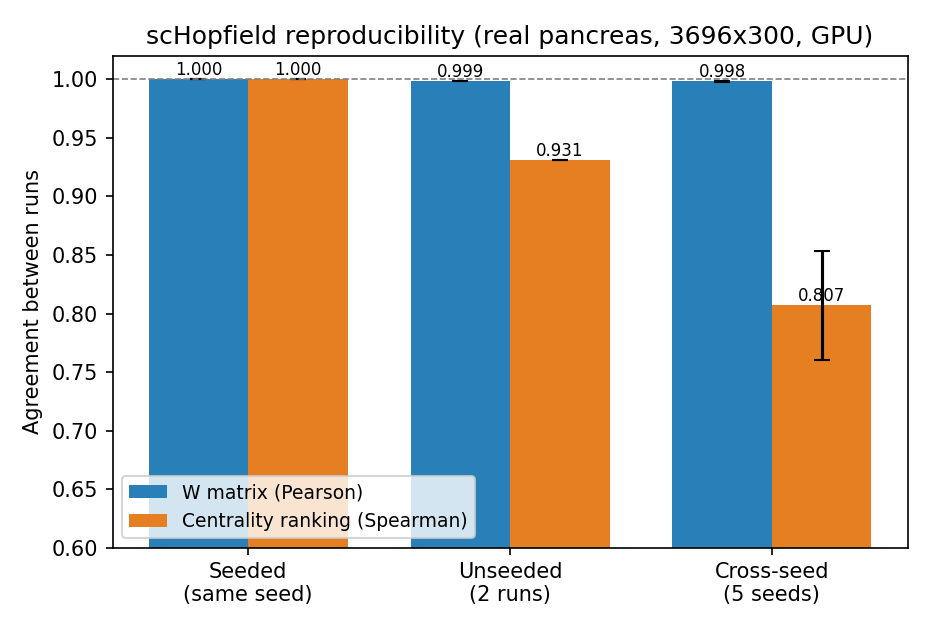
\includegraphics[width=0.7\linewidth]{figures/supp_repro.png}
\caption{Reproducibility of seeded vs unseeded inference (benchmark M1).}\end{figure}

\subsection*{S2. GRN recovery vs GENIE3}
On four synthetic 40-gene Hopfield networks with known ground truth, scHopfield recovered
edges at AUROC $0.975\pm0.018$ / AUPRC $0.970$ versus GENIE3 (expression-only ExtraTrees)
AUROC $0.701\pm0.025$ / AUPRC $0.240$ (benchmark M8).
\begin{figure}[htbp]\centering
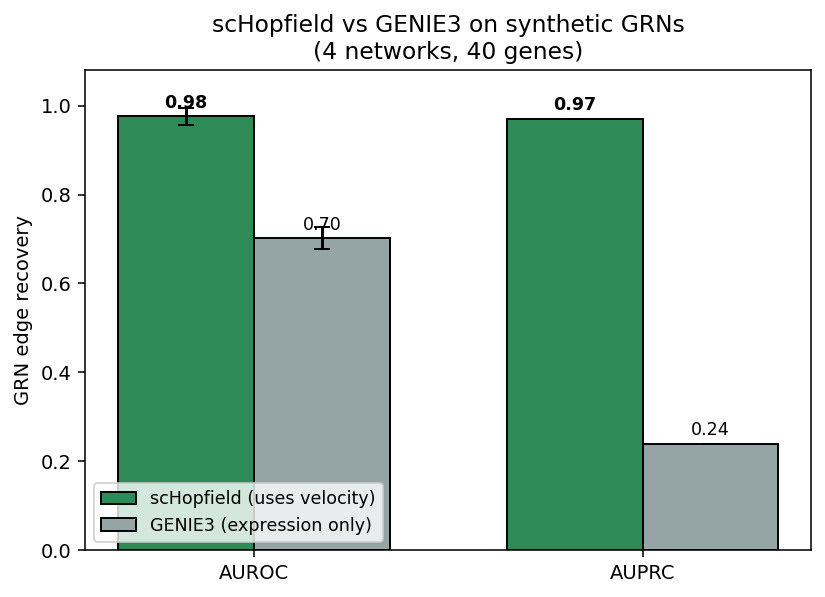
\includegraphics[width=0.55\linewidth]{figures/supp_genie3.png}
\caption{scHopfield vs GENIE3 GRN edge recovery.}\end{figure}

\subsection*{S3. Robustness of driver identification}
Across two mouse base networks and three scaffold-regularization regimes, perturbation-based
drivers were stable (mean pairwise Jaccard of top-15 genes 0.67) while the static network
score was unstable (0.20); an unconstrained pseudoinverse fit was an outlier (0.36) that
dropped Gata1/Klf1 (benchmarks M5, M6).
\begin{figure}[htbp]\centering
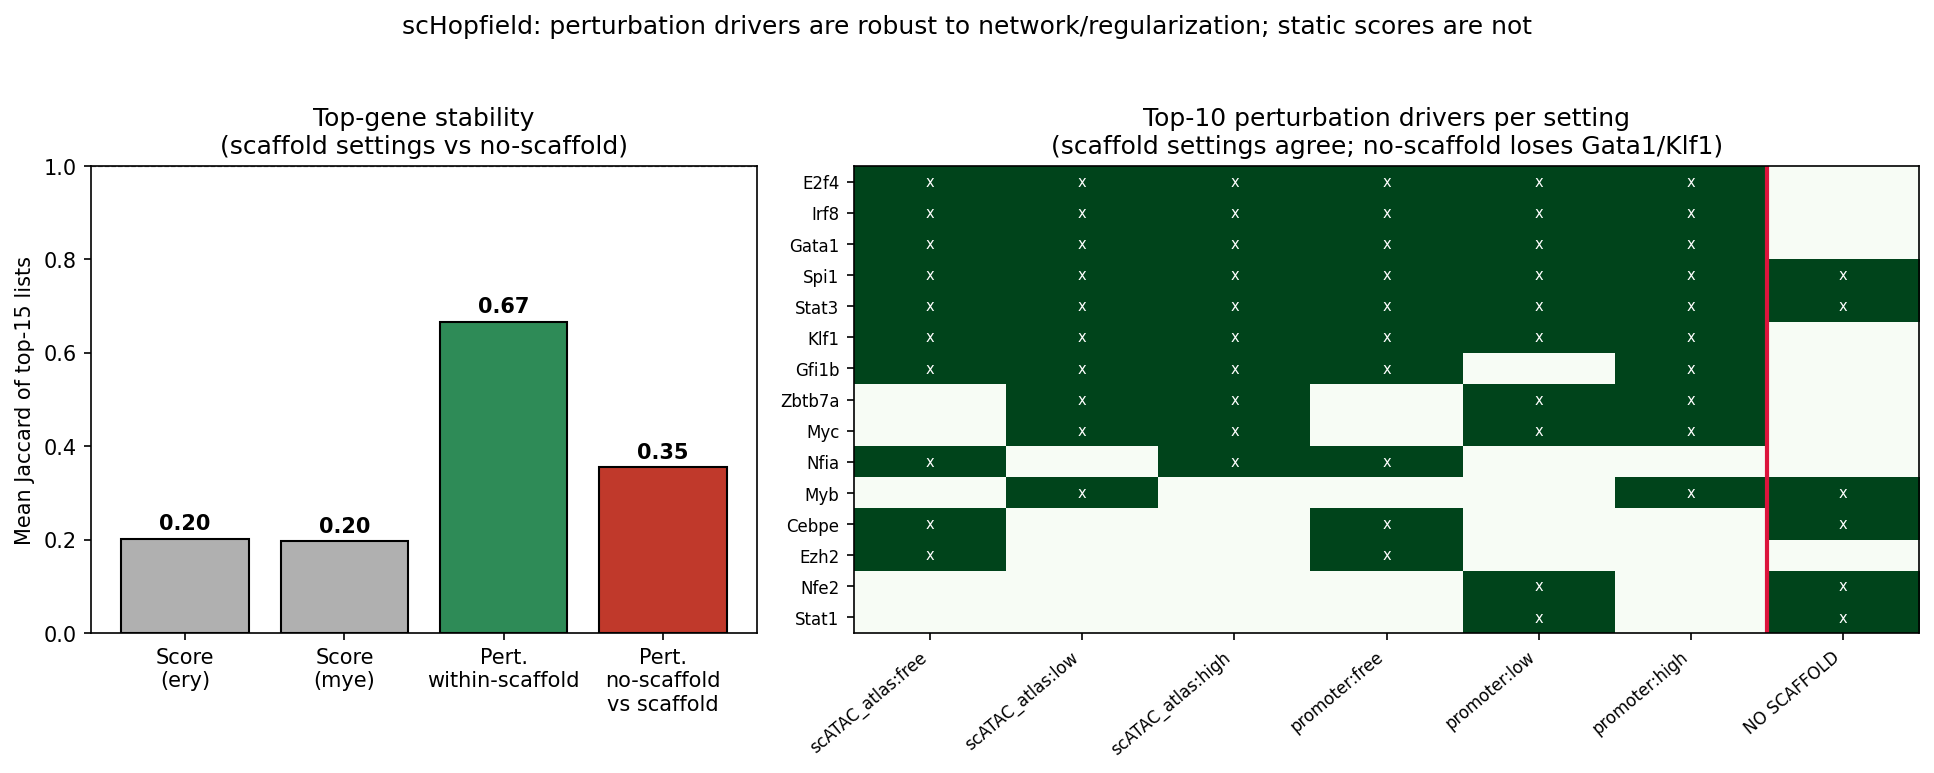
\includegraphics[width=0.9\linewidth]{figures/supp_sensitivity.png}
\caption{Network and regularization sensitivity of driver identification.}\end{figure}

\subsection*{S4. Biophysical circuits}
The dissertation oscillator is Hopfield-form and recovers at correlation 1.000. The Novak
cell-cycle and Adlung JAK-STAT circuits are not of Hopfield form (no true interaction
matrix) but the Hill model represents their velocity fields at $R^2=1.000$ (Hill-only basis
$R^2=0.98$/$0.99$); benchmark M9.

\subsection*{S5. Note on the Methods-equation Hill derivative}
The Hill derivative used in the Jacobian is $\varphi'(x)=n\,\varphi(1-\varphi)/x$; the
factor $n$ (present in the implementation) should be shown explicitly in Eq. (4) and
Eq. (21) (benchmark M2).

\end{document}
